% !TEX program = xelatex
\documentclass[a4paper,UTF8]{article}
\usepackage[version=4]{mhchem}
\usepackage[UTF8]{ctex}
\usepackage{fontspec}
\usepackage{geometry}
\usepackage{tcolorbox}
\usepackage{graphicx}
\setmainfont{SimSun}
\setlength{\parindent}{0em}
\setlength{\fboxsep}{1em}
\geometry{textwidth=15cm}
\geometry{hcentering}
\begin{document}
\begin{center}
{\huge 我的化学笔记}

\textbf{author:zzy}

按照第五版天津大学无机化学元素部分整理
\end{center}

\section{氢和稀有气体}
稀有元素:自然界中含量少和分布稀少,被人们发现较晚,难以从矿物中提取或是在工业上制备和应用较晚的元素
\subsection{稀有元素分类}
稀有元素:

(1)轻稀有元素:Li,Rb,Cs,Be

(2)分散性稀有元素:Ga,In,Tl,Se,Te

(3)高熔点稀有元素:Ti,Zr,Hf,V,Nb,Ta,Mo,W

(4)稀土元素:Sc,Y,La及镧系元素

\subsection{化合态和游离态}
游离态:

(1)气态非金属单质

(2)固态非金属单质

(3)金属单质

注:

过冷状态:液态物质在温度降低到凝固点而仍不发生凝固或结晶等相变的现象。(Cs,Ga)


\subsection{单质的制取方法}
1.物理分离法

淘洗黄金,分离氧气氮气

2.热分解法

热稳定性差的某些金属化合物直接加热

$$ \ce{2Ag2O ->[\Delta] 4Ag(s) + O2}$$
$$ \ce{HgS(s) + O2 ->[\Delta]  Hg(l) + SO2(g)}$$

热分解法还用于制备某些高纯单质

$$ \ce{Zr(\text{粗}) + 2I2 ->[600^\circ C] ZrI4 ->[1800^\circ C] Zr(\text{纯}) + 2I2} $$
3.还原法

使用还原剂制取单质的方法叫做还原法。

$$ \ce{MgO(s) + C ->[\Delta] Mg + CO ^}$$
$$ \ce{Fe2O3 + 2Al ->[\Delta] 2Fe + Al2O3} $$

4.电解法

活泼金属和非金属单质的制备可采用电解法。

$$ \ce{2Al2O3(\text{熔体}) ->[\text{电解}][Na3AlF4,960^\circ C] 3S + 2H2O} $$ 

5.氧化法

用氧化剂制取单质的方法。如制取S:

$$ \ce{3FeS2 + 6C + 8O2 ->[\Delta] Fe3O4 + 6CO2 ^ + 6S ^} $$

也可从\ce{H2S}制取S:

$$ \ce{2H2S + 3O2 -> 2SO2 + 2H2O} $$
$$ \ce{ 2H2S + SO2 ->[CaT][300^\circ C] 3S + 2H2O} $$

\subsection{氢}
\subsubsection{氢原子的成键效应}

1.失去价电子

\ce{H+}半径小,具有很强电场,极化作用很强。

2.结合一个电子

这是\ce{H}与活泼金属形成离子型氢化物如\ce{NaH}、\ce{CaH2}的成键特征

3.形成共价化合物

与其他非金属形成共价型氢化物(\ce{HCl}、\ce{H2S}、\ce{NH3})。

\subsubsection{氢的性质和用途}

性质:

1.溶解度:氢在水中溶解度很小,在金属中溶解度却很大。

2.活泼性:在常温下不活泼。原因是氢原子半径小,无内层电子,所以共用电子对直接受核作用,形成的$\sigma$键很牢固,\ce{H2}的解离能很大。

3.与金属:加热时,与碱金属、碱土金属化合形成离子型氢化物(性质见碱金属/碱土金属部分);\\在过渡型氢化物中,氢以三种形式存在:\\·原子状态存在于金属晶格中\\·氢的价电子进入氢化物导带,以\ce{H+}形式存在\\·氢从氢化物导带中得一个电子,以\ce{H-}形式存在\\高温下,\ce{H2}作为还原剂与氧化物或氯化物反应,还原某些金属和非金属。


用途:

氢的扩散性好,导热性强;熔沸点均低,难液化,可作超低温制冷剂;热值高可作高能燃料。

与碱金属、碱土金属化合形成离子型氢化物(性质见碱金属/碱土金属部分)

化工上,氢气和用于生产甲醇。
$$ \ce{CO(g) + 2H2(g) ->[\text{催化加压}][\text{加热}] CH3OH} $$

食品工业上,则可用于有机物催化加氢。


$$ \ce{WO3 + 3H2 ->[\text{高温}] W + 3H2O} $$
$$ \ce{SiHCl3 + H2 ->[\text{高温}] Si + 3HCl} $$

4.与非金属:绝大多数p区元素与\ce{H2}反应生成共价型氢化物,它们在固态多数属于分子晶体,故又称分子型氢化物;它们大多是无色的,熔沸点较低;它们的物理性质相似,但化学性质显著不同。

5.检验:氢气能让粉红色\ce{PdCl2}水溶液迅速变黑(析出金属钯粉)

$$ \ce{PdCl2(aq) + H2(g) ->[\text{高温}] Pd(s) v + 2HCl(aq)} $$

6.温度影响:高温下,氢分子分解为原子氢,具有极强还原性。

\subsubsection{氢气的制备}

实验室里,用\ce{Zn}与盐酸、稀硫酸作用制取氢气;

军事上使用\ce{CaH2}与水反应制取氢气。

工业上,主要有:

1.矿物燃料转化法:

制备水煤气:

$$ \ce{CH4(g) + H2O(g) ->[CaT][700-800^\circ C] CO(g) + 3H2} $$
$$ \ce{C(s) + H2O(g) ->[1000^\circ C] CO(g) + H2(g)} $$

将水煤气与水蒸气反应

$$ \ce{CO(g) + H2O(g) ->[400-600^\circ C][\ce{Fe},\ce{Cr}\text{催化剂}] CO2(g) + H2(g)} $$

本质上,每一步都是在让\ce{C}夺走水中的\ce{H}

该法制氢伴随大量\ce{CO2}产生。

2.电解法

电解\ce{NaOH}溶液,则在阴极产生氢气,阳极产生氧气。

\subsection{稀有气体}

稀有气体:0族元素所对应的气体单质。

\subsubsection{稀有气体的性质和用途}

稀有气体原子间存在微弱的色散力,作用力随着原子序数增大而增大(因为分子变形性增大)。所以,稀有气体的物理性质(熔沸点、临界温度、溶解度)也随着原子序数增大而增大。

1.氦(\ce{He})

用来代替氧气瓶中\ce{N2},防止潜水员“潜水病”。

2.氖(\ce{Ne})和氩(\ce{Ar})

霓虹灯、保护气、冷冻剂。

3.氪(\ce{Kr})和氙(\ce{Xe})

特种光源、麻醉剂。

4.氡(\ce{Rn})

有放射性,可用于放疗。

\subsubsection{稀有气体化合物}
第一个稀有气体化合物:

$$ \ce{Xe(g) + PtF6(g) -> Xe+[PtF6]-(s)} $$

现在,有稀有气体卤化物、氧化物、含氧酸盐等,大多都与氟化物的反应有关。

稀有气体氟化物:

$$ \ce{Xe(g) + F2(g) -> XeF_{x}(g)} $$

根据\ce{F}的用量和时间长短,可分别制得$x=2,4,6$的化合物;反应中若进入湿气,则生成爆炸的\ce{XeO3}。

\ce{XeF2}与水反应生成\ce{Xe}和\ce{HF}、\ce{O2};\ce{XeF4}、\ce{XeF6}则与水反应生成固态的\ce{XeO3}

\ce{Xe}的氟化物是优良的氟化剂,如:

$$ \ce{Pt + XeF4 -> PtF4 + Xe} $$

\ce{Xe}的三种氟化物均为强氧化剂,如:

$$ \ce{XeF2 + H2O2 -> Xe + 2HF + O2 ^} $$

$$ \ce{6HCl + XeF6 -> 3Cl2 ^ + 6HF + Xe} $$

$$ \ce{6HCl + XeF6 -> 3Cl2 ^ + 6HF + Xe} $$

需要注意的是\ce{Xe}的氟化物的分子结构。\ce{XeF4}中有中心原子的8个电子,每个\ce{F}原子提供一个价电子,价层有$\frac{8+(4\times1)}{2}=6$对电子,为八面体结构。两对孤电子占据对角,四个成键电子对占据四个顶点,为正方形,\ce{Xe}位于正方形中心。



\section{碱金属和碱土金属元素}

\subsection{碱金属和碱土金属通性}

$IA$和$IIA$族元素均只有1到2个s电子,同一周期中,半径大、电荷少。所以,它们的金属晶体中金属键不牢固,单质熔沸点低,硬度小。由于碱土金属比碱金属原子半径小、原子电荷多,因此碱土金属的熔沸点都比碱金属高,密度、硬度都比碱金属大。

总的来说,从上到下熔沸点降低、密度增加、硬度减小、电负性降低、$E^{\theta}(\ce{M2+}/\ce{M})$绝对值增加,还原性增加。

然而,\ce{Li/Li+}的标准电极电势反常,这是因为其原子半径小,很容易与\ce{H2O}结合放出能量,水合焓代数值最小导致的。研究反应的焓变,可以得到如下过程。

\begin{figure}[htpb]
	\centering
	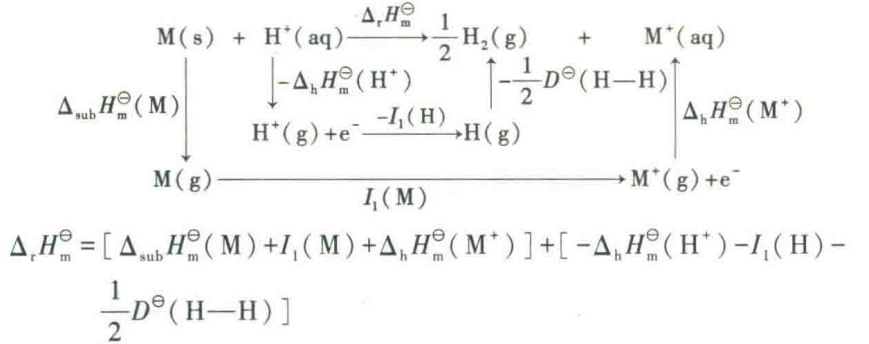
\includegraphics[width=0.8\textwidth]{figure//Li的电极电势反常的原因.png}
	\caption{Li的水合焓对焓变的影响}
	\label{fig:}
\end{figure}

\begin{tcolorbox}

%\begin{figure}[htpb]
%	\centering
%	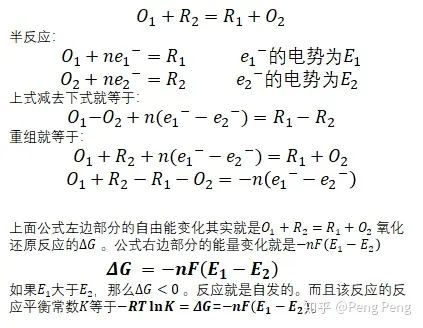
\includegraphics[width=0.5\textwidth]{figure//电势与Gibbs自由能.png}
%	\caption{电势与Gibbs自由能的关系}
%	\label{fig:}
%\end{figure}

如何描述Gibbs自由能与电势的关系:

例如,对于反应

$$ \ce{O1 + R2 = R1 + O2} $$

半反应:

$$ \ce{O1 + ne1^- = R1 \quad potential\ of\ e1^- = E_1} $$

$$ \ce{O2 + ne2^- = R2 \quad potential\ of\ e2^- = E_2} $$

上式减下式就等于(注意,此处从左到右均为还原反应):

$$ \ce{O1 - O2 + n(e1^- - e2^-) = R1 - R2} $$

重组就等于:

$$ \ce{O1 + R2 - R1 - O2 = -n(e1^- - e2^-)} $$

上面公式左边部分的变化就是 $ \ce{O1 + R2 = R1 + O2} $ 氧化还原反应的 $ \Delta G $。公式右边部分的能量变化就是$ -nF(E_1 - E_2) $

$$ \ce{\Delta G = -nF(E1 - E2)} $$

若$ E1 > E2 $,那么$ \Delta G < 0 $。反应就是自发的。而且反应平衡常数有 $ -RTlnK = \Delta G = -nF(E1 - E2) $值得注意的是,此处$E_1$为原反应的还原部分,而$E_2$为氧化部分。\\

电动势的本质,就是两个电极之间各物质的电化学势能(electromical potential)总和达到平衡,测量出的电子在两端电极的电势能之差。

关于电化学势能,它与物质的活度、带电荷数有关。

\end{tcolorbox}

碱金属和碱土金属均可溶于液氨,生成溶剂合电子和阳离子,形成具有导电性的深蓝色溶液。

$$ 碱金属:\ce{M(s) + (x + y)NH3 <=> M+(NH3)_x + e^-(NH3)_y}(蓝色) $$

$$ 碱土金属:\ce{M(s) + (x + 2y)NH3 <=> M^2+(NH3)_x + 2e^-(NH3)_y}(蓝色) $$

碱金属、碱土金属的氨溶液具有导电性,可发生于金属本身类似的化学反应,例如钾的液氨溶液可还原\ce{Ni(II)},制得\ce{Ni(I)}配合物:

$$ \ce{2K2[Ni(CN)4] + 2K+(NH3) + 2e^-(NH3) ->[-30^\circ C below][NH3(l)] K4[Ni2(CN)6](NH3)4 + 2KCN} $$

碱金属和碱土金属氨溶液不稳定,可以被催化为氨基化物(阳离子与氨基连接):

$$ \ce{Na+(NH3) + e^-(NH3) ->[FexOy] NaNH2(NH3) + \frac{1}{2}H2(g)} $$

碱金属可以溶于醚和烷基胺中。

碱金属和碱土金属可以与\ce{H2,H2O,X2,N2,S,O2}反应,其中与\ce{N2}反应的有\ce{Li,Mg,Ca,Sr,Ba};与\ce{H2O}反应的有碱金属,\ce{Ca,Sr,Ba,Mg}。

\subsection{氢化物}

碱金属和碱土金属加热时与氢直接化合,形成离子型氢化物,其中氢为-1价。

所有纯的离子型氢化物都是白色晶体,不纯的为浅灰色至黑色。性质类似盐,又称为类盐型氢化物,密度比相应金属密度大得多。

类盐型氢化物:碱金属和碱土金属与氢化合形成的离子型氢化物。

离子型氢化物受热分解为氢气和游离金属。

$$ \ce{2MH ->[\Delta] 2M + H2 ^} $$

离子型氢化物与水反应生成氢气,原因是\ce{H-}与水中\ce{H+}结合为\ce{H2}。

$$ \ce{LiH + H2O -> LiOH + H2 ^} $$

离子型氢化物都是极强的还原剂,其电对电势可达-2.23V。

有些氢化物在干燥空气中稳定,其他的会自燃。

\ce{LiH}能在乙醚中同\ce{B^3+,Al^3+,Ca^3+}等的无水氯化物结合形成复合氢化物:

$$ \ce{4LiH + AlCl3 ->[\text{乙醚}] Li[AlH4] + 3LiCl} $$

氢化铝锂遇水剧烈反应:

$$ \ce{Li[AlH4] + 4H2O -> LiOH v + Al(OH)3 v + 4H2 ^} $$

\subsection{氧化物}

碱金属和碱土金属能形成多种类型的氧化物,正常氧化物(\ce{O^2-})、过氧化物(\ce{O2^2-})、超氧化物(\ce{O2^-})、臭氧化物(\ce{O3^-})、低氧化物。

s区元素形成的氧化物中,

在空气中直接形成正常氧化物:\ce{Li}与碱土金属;

在空气中直接形成过氧化物:\ce{Na};

在空气中直接形成超氧化物:\ce{Na,K,Rb,Cs};

不能形成过氧化物:\ce{Be};

不能形成超氧化物:\ce{Li,Be,Mg}。

\subsubsection{正常氧化物}

如之前所说,Li与所有碱土金属在空气中燃烧生成正常氧化物。其他碱金属的正常氧化物需要用它们的过氧化物或硝酸盐与金属反应制得。

$$ \ce{Na2O2 + 2Na -> 2Na2O} $$

$$ \ce{2KNO3 + 10K -> 6K2O + N2 ^} $$

或者也可以用它们的碳酸盐或硝酸盐加热分解得到。

$$ \ce{CaCO3 ->[\Delta] CaO + CO2 ^} $$

$$ \ce{2Sr(NO3)2 ->[\text{强热}] 2SrO + 4NO2 ^ + O2 ^} $$

一些碱金属氧化物的颜色:

\ce{Li2O,Na2O}:白色;

\ce{K2O}:淡黄色;

\ce{Rb2O}:亮黄色;

\ce{Cs2O}:橙红色。

碱土金属氧化物则均为白色粉末。

碱土金属氧化物在水中溶解度较小,除了\ce{BeO}为\ce{ZnS}型晶体外,其余都为\ce{NaCl}型晶体。它们的硬度和熔点都很高。

\subsubsection{过氧化物和超氧化物}

过氧化物可看做\ce{H2O2}的衍生物,含有过氧基(\ce{---O---O---})。

\ce{Li,Be,Mg}之外的碱金属和碱土金属都存在超氧化物,\ce{Na,K,Rb,Cs}在过量氧气中燃烧直接生成超氧化物。

\ce{Na2O2}的制备:工业上用熔钠与压缩空气(除\ce{CO2})反应,实验室中用饱和\ce{NaOH}溶液与一定浓度\ce{H2O2}反应。

$$ \ce{2NaOH + H2O2 ->[0^\circ C] Na2O2 + 2H2O} $$

\ce{Na2O2}在碱性介质中为强氧化剂,例如可将\ce{CrO2^-}氧化为\ce{CrO4^2-}。

室温下,过氧化物、超氧化物与水或稀酸反应生成过氧化氢(和氧气),过氧化氢又分解放出氧气。

$$ \ce{Na2O2 + 2H2O -> 2NaOH + H2O2} $$

$$ \ce{2KO2 + H2O -> 2KOH + H2O2 + O2 ^} $$

过氧化物与超氧化物与二氧化碳反应放出氧气。

$$ \ce{2Na2O2 + 2CO2 -> 2Na2CO3 + O2 ^} $$

$$ \ce{4KO2 + 2CO2 -> 2K2CO3 + 3O2 ^} $$

\subsubsection{臭氧化物}

低温下,\ce{O3}与粉末状无水碱金属(除Li)氢氧化物反应,并用液氨提取,可得到红色\ce{MO3}固体。

$$ \ce{3MOH(s) + 2O3(g) -> 2MO3(s) + MOH * H2O(s) + \frac{1}{2}O2(g)} $$

室温下,臭氧化物缓慢分解为\ce{MO2}和\ce{O2};

臭氧化物与水反应:生成\ce{MOH}和\ce{O2}。

\subsection{氢氧化物}

碱金属、碱土金属的氧化物(除\ce{BeO,MgO}之外)与水反应即可得到相应氢氧化物和大量热。

均为白色固体,易潮解,在空气中吸收\ce{CO2},生成碳酸盐。

苛性碱:碱金属氢氧化物。

\subsubsection{碱金属和碱土金属氢氧化物的碱性}

碱金属和碱土金属氧化物(除了\ce{Be(OH)2}外)均呈碱性,同族元素碱性随着原子序数增加而增强。

\ce{Be(OH)2}:两性氢氧化物,既溶于酸也溶于碱。

$$ \ce{H2BeO2 + 2OH- -> BeO2^2- + 2H2O} $$

或

$$ \ce{Be(OH)2 + 2OH- -> [Be(OH)4]^2-} $$

\begin{tcolorbox}

在水中,\ce{R-O-H}有两种解离方式:

$$ \ce{(\text{酸式解离}) RO- + H+ <- R-O-H -> R+ + OH- (\text{碱式解离})} $$

可以通过离子势衡量阳离子极化作用强弱,来判断解离方式。

$$ 离子势(\Phi) = \frac{阳离子电荷(z)}{阳离子半径(r)} $$

若R的$\Phi$大,则R的电场强,极化作用强,O电子云偏向R,令\ce{O-H}键被削弱,按酸式解离,否则按碱式解离。

一般以$ \sqrt{\Phi} $作为酸碱性依据,分界点为0.22,0.32。

\end{tcolorbox}

\subsection{盐类}

\subsubsection{盐类性质}

1.晶体类型

大多数碱金属、碱土金属的晶体属于离子晶体(除\ce{Be^2+},其半径小、电荷多,极化力强,与除\ce{F-}的卤素结合生成共价晶体)。

2.颜色

碱金属和碱土金属盐的颜色通常显阴离子颜色,如\ce{CrO4^2-}盐为黄色,\ce{MnO4-}盐为紫红色。

焰色反应:碱金属和碱土金属化合物在高温火焰中部分电子获得能量激发到高能级轨道上,而电子从高能级轨道回到 低能轨道时,将发出某种特定波长的光,使火焰呈现特征颜色。

$ Li:深红 \quad Cs:蓝 $

$ Na:黄 \quad Ca:橙红 $

$ K:紫 \quad Sr:洋红 $

$ Rb:紫红 \quad Ba:绿 $

3.热稳定性

对于碱金属:

卤化物:高温时挥发不分解

硫酸盐:高温既不挥发也不分解

碳酸盐:高温不分解(除\ce{Li2CO3}部分分解)

硝酸盐:加热到一定温度分解,生成氧化物、\ce{NO2}和氧气(对于\ce{LiNO3})或者亚硝酸盐和氧气。

碱土金属的碳酸盐常温下稳定(除\ce{BeO2}),强热时分解。

4.溶解度

碱金属盐类易溶于水。除了若干锂盐和钾铷铯与复杂阴离子形成的盐。

e.g.\ce{LiF,Li2CO3,Li3PO4,KClO4,K2PtCl6},etc.

碱土金属中,铍盐大多易溶,镁盐部分易溶,钙、锶、钡盐多难溶。

随着\ce{Ca-Sr-Ba}的顺序,硫酸盐、铬酸盐溶解度递减,氟化物溶解度递增。

铍盐和可溶性钡盐有毒。

5.鉴定

\begin{tabular}{c|c|c}
	离子&鉴定试剂&鉴定现象\\ \hline
	\ce{Na+}&\ce{KH2SbO4}&产生白色沉淀\\
	\ce{K+}&\ce{Na3[Co(NO2)6]^3-}&产生亮黄色沉淀\\
	\ce{Mg^2+}&镁试剂&产生天蓝色沉淀\\
	\ce{Ca^2+}&\ce{(NH4)2C2O4}&产生白色沉淀\\
	\ce{Ba^2+}&\ce{K2CrO4}&产生黄色沉淀\\
\end{tabular}

\subsubsection{盐类的生产}

1.碳酸钠:

氨碱法(侯德榜制碱法):煅烧碳酸钙得到\ce{CO2},将其与氨一起通入饱和的\ce{NaCl}食盐水中,析出\ce{NaHCO3},再进行煅烧得到碳酸钠。

$$ \ce{NaCl + NH3 + CO2 + H2O ->[\text{冷}] NaHCO3 + NH4Cl} $$

2.硫酸钙

石膏:二水硫酸钙

熟石膏:半水硫酸钙

工业上的制备:

$$ \ce{CaCl2 + (NH4)2SO4 + 2H2O -> CaSO4 * 2H2O + 2NH4Cl} $$

\subsection{配合物}

碱金属离子由于电荷少,半径大,不容易形成配合物。只有与配位能力强的螯合剂作用才会形成配合物(螯合物或大环配合物)。

碱土金属和碱金属可与冠醚形成配合物,例如叶绿素。

\section{卤素和氧族元素}

\subsection{p区元素概述}

p区元素具有以下特点

(1)从上到下原子半径逐渐增大,金属性逐渐增强,非金属性逐渐减弱。

(2)p区元素的价电子构型为$ ns^2np^{1-5} $。ns,np电子均可参与成键,氧化数较多,且有正有负。

惰性电子对效应:$ IIIA \sim VA $ 族同族元素从上到下低氧化数化合物的稳定性增强,高氧化数化合物的稳定性减弱。

(3)p区金属的熔点一般较低。

(4)p区某些金属具有半导体性质。

\subsection{卤族元素}

\subsubsection{卤族元素通性}

卤素:VIIA族元素。

卤素的核电荷数是同周期中最多的,原子半径是同周期中最小的,它们最容易取得电子。

卤素的第一电离能都很大,一般不会失去电子(碘除外,可以形成碘(III)盐,如\ce{I(ClO4)3})。

除了失去电子的情况以外,卤素若与电负性大的元素化合,可以可以表现出正氧化数,且相邻氧化数的差均为2。这是因为卤素有一个电子未成对,参加反应后每拆开一个电子对形成两个共价键。

\subsubsection{卤素单质}

1.物理性质

熔沸点:卤素固态为非极性晶体,熔沸点低,且从上到下递增(原因:原子r和z增加,色散力增大)。\\

颜色:卤素单质有颜色,且逐渐加深:

\begin{center}

\begin{tabular}{c|c}
	单质&颜色\\ \hline
	氟&浅黄\\
	氯&黄绿\\
	溴&红棕\\
	碘&紫黑\\
\end{tabular}

\end{center}

溶解度:卤素在水中溶解度不大(F与水激烈反应),在有机溶剂中溶解度较大。

碘难溶于水,但易溶于碘化物溶液,这是因为:

$$ \ce{I2 + I- <=> I3^-(\text{黄色或棕色})} $$

此反应是因为\ce{I-}接近\ce{I2},使\ce{I2}极化产生诱导偶极,彼此由于静电吸引。

气味:均有刺激性气味,有毒。

液溴灼烧皮肤,若溅到身上,立即用大量水冲洗再用\ce{NaHCO3}溶液淋洗。\\

2.化学性质:\\

最突出的是氧化性。\ce{F2}是最活泼的非金属,是卤素单质中最强的氧化剂。从上到下氧化能力减弱。

(1)卤素与单质反应:\ce{F2}阴冷条件遇氢爆炸,\ce{Cl2}强光下遇氢爆炸。

氟易氧化所有金属和除氮、氧和某些稀有气体以外的非金属单质,并且十分激烈。但氟与铜、镍作用会形成金属氟化物保护膜,可用于储存氟。氯在干燥时则不与铁反应。\\

(2)卤素与水反应:

第一类:氧化作用:

$$ \ce{2X2 + 2H2O -> 4HX + O2 ^} $$

第二类:水解(歧化)作用:

$$ \ce{X2 + H2O -> H+ + X- + HXO} $$

\ce{F2}只与水发生第一类反应;\ce{Cl2}在日光下缓慢置换水中的氧气;\ce{I-}反而会被氧气氧化。

\ce{Cl2,Br2,I2}主要与水发生第二类反应,此时反应可逆,反应进行程度从上到下越来越小。加酸抑制水解,加碱促进水解。\\

(3)卤素的制备:

总的来说是卤素阴离子的氧化。

\ce{F2}:\ce{F-},采用电解法或\ce{K2MnF6}氧化。

\ce{Cl2}:电解饱和食盐水;实验室里用\ce{MnO2,KMnO4,K2CrO7,KClO3}等与浓\ce{HCl}反应。

\ce{Br2}:用氯气氧化溴离子;工业上要先用氯气吹出\ce{Br2},用\ce{Na2CO3}吸收富集,

$$ \ce{3CO3^2- + 3Br2 -> 5Br- + BrO3- + 3CO2 ^} $$

再用硫酸酸化,令\ce{Br}归中。

\ce{I2}:用氯气将碘从海带或卤水中置换出来,或用\ce{HSO3-}还原碘酸根。\\

用途:(P259)

氟用于制备六氟化铀,用于富集核燃料;含氟化合物很稳定,聚四氟乙烯、氟化烃、全氟烃、氟化石墨、氟化物玻璃。

氯用于合成盐酸、聚氯乙烯、漂白粉、塑料、橡胶等。

溴用于燃料、感光材料,在医药中可用于镇静剂和安眠药。

碘化物是重要的化学试剂;在医药上用作消毒剂;碘仿(\ce{CHI3})用作防腐剂,添加\ce{KIO3}的碘盐等。

\subsubsection{卤化氢和氢卤酸}

1.制备:\\

氯化氢:直接合成法(\ce{H2 + Cl2})。\\

氟化氢(或少量氯化氢):卤化物与浓硫酸反应(生成硫酸氢盐和卤化氢),如:

$$ \ce{CaF2 + 2H2SO4(\text{浓}) -> Ca(HSO4)2 + 2HF ^} $$

溴化氢、碘化氢:非金属卤化物水解,如:

$$ \ce{3Br2 + 2P + 6H2O -> 2H3PO3 + 6HBr ^} $$

本质上,是利用卤素氧化非金属形成易酸性水解的阴离子,生成\ce{H+}与\ce{Br-}结合。

2.性质\\

物理性质:

卤化氢具有强烈刺激性,是无色气体,空气中形成白色酸雾。

卤化氢是极性分子,极易溶于水。

氢卤酸:卤化氢的水溶液。

浓的氢卤酸打开瓶盖就冒烟。

除了\ce{HF}外,其余卤化氢性质按照卤素从上到下顺序熔沸点升高、生成焓升高、溶解度升高。\\

化学性质(注意\ce{HF}的特殊性):

(1)酸性:氢卤酸中,从氯到碘均为强酸且酸性,且从上到下逐渐增强(原理:半径增大,卤素原子对氢原子的吸引力减小,更加容易失去,酸性加强);

氢卤酸中只有氢氟酸为弱酸,但浓度高时变为强酸,原因是生成了缔合离子\ce{HF2-,H2F3-}等,消耗了\ce{F-},令\ce{HF}解离正向进行。

$$ \ce{F- + HF <=> HF2-} $$

\begin{tcolorbox}

氢氟酸是弱酸的原因:

从热力学上看,这是因为在\ce{HX}中,\ce{HF}解离过程中焓变的代数值最大(放热最少)。这是因为\ce{H-F}键解离能大,脱水焓小(因为\ce{HF}溶液中存在氢键),且\ce{F}的电子亲和能偏高。

从结构上看,\ce{HF}中氢、氟原子半径小,吸引\ce{H+}的能力很强,不易解离。

\end{tcolorbox}

(2)还原性:\ce{F,Cl}较难被氧化,但溴化氢和碘化氢溶液容易变为棕色。\\

(3)热稳定性:热稳定性随着卤素元素从上到下急剧下降,\ce{HI(g)}在$ 200^\circ C $明显分解。\\

3.用途:\ce{HF}可用于腐蚀玻璃等。

$$ \ce{SiO2 + 4HF -> SiF4 ^ + 2H2O} $$

\subsubsection{卤化物}

1.键型

卤化物化学键类型与成键元素的电负性、原子或离子的半径、金属离子的电荷有关。

离子型卤化物具有熔沸点高、挥发性低、熔融导电的特性;共价型卤化物熔沸点低、会挥发、熔融不导电;但二者没有明显的界限,如\ce{FeCl3}为共价型,易挥发但熔融导电。

碱金属和碱土金属(除Li,Be)和大多镧系、锕系的卤化物基本上是离子化合物;随着金属离子半径的减小、离子电荷的增加和卤素离子半径的增大,键型由离子向共价型过渡的趋势增强。\\

2.溶解度

大多数卤化物易溶于水,除了\ce{AgX,PbX2,Hg2X2,CuX}是难溶的。

但是\ce{F}的情况有所不同,相同阴离子的卤化物中,仅有\ce{CaF2}难溶、\ce{AgF}易溶。

\begin{tcolorbox}

\ce{F}的卤化物反常原因:

主要是因为\ce{F-}半径过小。对于\ce{Ca^2+}来说,\ce{F-}半径小,与\ce{Ca^2+}吸引力强,令\ce{CaF2}的晶格能大,难溶;对于\ce{Ag+}来说,其极化力和变形性都大,但\ce{F-}半径小,难以被极化,\ce{Ag-F}键主要为离子型,溶解度大。

总的来说,对于电荷多的离子,\ce{F-}吸引力强导致晶格能大而相对难溶;对于极化力强的离子,\ce{F-}难以被极化导致共价性小而相对易溶。

\end{tcolorbox}

2.金属卤化物的制备\\

(1)湿法:用金属或金属氧化物、氢氧化物、碳酸盐与酸或酸和氧化剂反应,可制得相应金属氯化物。

$$ \ce{Cu + H2O2 + 2HCl -> CuCl2 + 2H2O} $$

(2)干法:强烈水解的氯化物(\ce{SnCl4,SiCl4}等)只能采用干法。用元素单质与氯气直接反映制得氯化物,但要及时分离产品。对于氧化物来说,实质上是氯气置换出氧气。\\

\subsubsection{氯的含氧酸及其盐}

1.概述

卤素(除氟)均可形成正氧化数的含氧酸,如:

\begin{tabular}{c|c|c|c|c}
	氧化数&氯&溴&碘&名称\\ \hline
	+1&\ce{HClO}&\ce{HBrO}&\ce{HIO}&次卤酸\\
	+3&\ce{HClO2}&\ce{HBrO2}&-&亚卤酸\\
	+5&\ce{HClO3}&\ce{HBrO3}&\ce{HIO3}&卤酸\\
	+7&\ce{HClO4}&\ce{HBrO4}&\ce{HIO4,H5IO6}&高卤酸\\
\end{tabular}

卤素的含氧酸中,氧的数量等于(氧化数+1)/2;反过来说氧化数等于氧的数量*2-1。

卤素的含氧酸不稳定,许多都只能存在于水溶液中。

几乎所有$E_A^\Theta(X_2/X-)$都有较大正值,表明在酸性溶液中卤素单质及其含氧酸均有较强氧化性,还原产物一般为\ce{X-}。

许多中间氧化数物质由于$ E_右^\Theta > E_左^\Theta $,存在发生歧化反应可能性。

\begin{tcolorbox}

	$E_A^\Theta(X_2/X^-) = E_B^\Theta(X_2/X^-)$的原因:

	电极电势与参与反应的物质浓度有关:(P96重要)

	$ E = E^\Theta + \frac{RT}{zF} ln(\frac{氧化型}{还原型}) $

	单质的氧化还原反应不涉及\ce{H+,OH-},所以相等;含氧酸的氧化还原反应涉及\ce{H2O},所以不同。

\end{tcolorbox}

2.次氯酸及其盐

\ce{Cl2}在水或碱中水解歧化生成\ce{HClO},加入可与\ce{HCl}反应的物质可使反应进行程度加大。

\ce{2Cl2 + 2HgO + H2O -> HgO * HgCl2 v + 2HClO}

次氯酸比碳酸弱,不稳定,易分解:

$$ \ce{2HClO ->[light] 2HCl + O2 ^} (分解)$$

$$ \ce{3HClO ->[\Delta] 2HCl + HClO3} (歧化)$$

$$ \ce{2HClO ->[\text{脱水剂}] Cl2O + H2O} (脱水) $$

漂白粉是次氯酸盐(有效成分)和碱式氯酸盐的混合物。其制备方法是:

$$ \ce{2Cl2 + 3Ca(OH)2 -> Ca(ClO)2 + CaCl2 * Ca(OH)2  * H2O + H2O} $$

使用时,用稀酸处理,如通入\ce{CO2}:

$$ \ce{Ca(ClO)2 + CaCl2 * Ca(OH)2  * H2O + 2CO2 -> 2CaCO3 v + 2HClO + CaCl2 + H2O} $$

(\ce{CO2}反应掉\ce{Ca(OH)2}和一个\ce{H2O},提供一个水两个氢离子)\\

3.氯酸及其盐

用氯酸钡与稀硫酸反应可制得氯酸溶液:

$$ \ce{Ba(ClO3)2 + H2SO4 -> BaSO4 v + HClO3} $$

氯酸含量高于$40\%$就会分解甚至爆炸,生成高氯酸、氯气、氧气:

$$ \ce{HClO3 -> HClO4 + Cl2 ^ + O2 ^ + H2O} $$

氯酸是强酸,可将碘(红棕色)氧化为碘酸(无色),同时生成氯气(黄绿色气体):

$$ \ce{2HClO3 + I2 -> 2HIO3 + Cl2 ^ (\text{黄绿色})} $$

氯酸钾在有催化剂时加热时分解为氯化钾和氧气:

$$ \ce{KClO3 ->[MnO2] 2KCl + 3O2 ^} $$

加热时无催化剂则分解为高氯酸钾(白色粉末)和氯化钾:

$$ \ce{4KClO3 -> 3KClO4 + KCl} $$

固体氯酸钾是强氧化剂,与还原性物质或有机物、可燃物混合产生燃烧和爆炸,制造火柴烟火等。

氯酸盐在酸性溶液中显示氧化性,例如\ce{KClO3}在中性溶液不能氧化\ce{KI}但在酸性中可以。

制备氯酸钾通常使用电解法。\\

4.高氯酸及其盐

浓硫酸与高氯酸钾作用可制备高氯酸。

工业上电解氧化氯酸盐制备高氯酸。\\

无水高氯酸是无色、微发烟液体,受热分解:

$$ \ce{4HClO4 ->[\Delta] 2Cl2 ^ (\text{黄绿色}) + 7O2 ^ + 2H2O} $$

酸性:高氯酸是常见的最强无机酸。

稳定性:高氯酸盐较稳定,例如\ce{KClO4}热分解温度大于\ce{KClO3}。

溶解性:高氯酸盐一般可溶,但与吸引力强的离子如\ce{K+,Rb+,Cs+,NH4+}的高氯酸盐晶格能大,难溶。除此之外,无水高氯酸镁可作高效干燥剂。

5.总结

氯的含氧酸及其盐的氧化型、热稳定性、酸性的一般规律总结:

\begin{figure}[htpb]
	\centering
	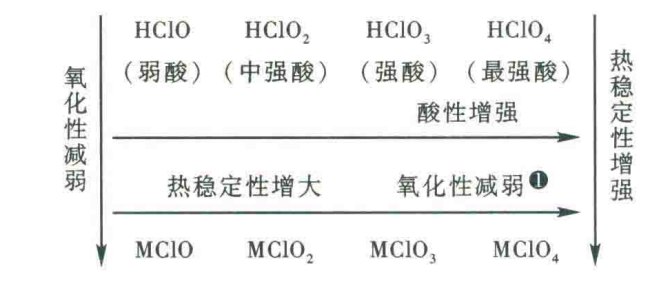
\includegraphics[width=0.8\textwidth]{figure//变化规律.png}
	\caption{其中氧化性HClO2表现不规则}
	\label{fig:}
\end{figure}

\begin{tcolorbox}

	含氧酸中非羟基氧的个数越多,氧化型越强。

\end{tcolorbox}

\subsubsection{拟卤素}

拟卤素:某些原子团形成的分子、离子分别与卤素单质、离子有着相似的性质,称为拟卤素。

重要的拟卤素有\ce{(CN)2,(SCN)2,(OCN)2}。

\subsection{氧族元素}

氧族元素:周期第VIA族,氧,硫,硒,碲,钋,鉝。

氧族元素从上往下原子半径和离子半径逐渐增大,电离能和电负性逐渐变小;金属性增强,非金属性减弱。

氧族元素价层电子构型为$ns^2np^4$,其原子有获得两个电子的趋势,表现较强的非金属性。

化学键类型:氧在VIA族电负性最大,与大多数金属离子形成二元离子化合物;硫、硒、碲与大多数金属化合形成共价化合物。

\begin{tcolorbox}

	为什么VIA族只有氧无正氧化数:

	因为硫、硒、碲存在可利用的d层轨道,可形成+2,+4,+6的化合物,但氧没有。

\end{tcolorbox}

\subsubsection{氧和臭氧}

1.氧

氧分子解离能较大,常温下反应性能较差。但加热时除了卤素和少数贵金属(\ce{Au,Pt})及稀有气体,几乎可与所有元素直接化合为相应的氧化物。\\

2.臭氧

臭氧分子形成\ce{\Pi_3^4},无单电子,为反磁性物质。

\begin{tcolorbox}

形成大$\Pi$键的条件:

1.原子位于同一平面上;

2.原子有一相互平行的p轨道;

3.p轨道数目的两倍大于p电子数。

\end{tcolorbox}

$\Delta$鉴别\ce{O3},在碘化钾溶液中使碘析出:

$$ \ce{O3 + 2I- + 2H+ -> I2 + O2 ^ + H2O} $$

\subsubsection{水}

羟基水:在化合物中以\ce{OH-}的形式存在的水。

配位水:在化合物中以配体形式存在的水。

阴离子水:通过氢键与阴离子结合的水,如\ce{CuSO4 * 5H2O}中4个水分子为配位水,一个为阴离子水。

晶格水:位于水合物晶格中的水,不与阴阳离子直接连接,如\ce{MgSO4 * 7H2O}中有1个为晶格水。

沸石水:在某种物质的晶格中占据相对无规律的位置,加热脱除时物质的晶格不被破坏。

\subsubsection{过氧化氢}

过氧化氢:近乎无色的粘稠液体,分子间有氢键,沸点比水高。\\

1.性质:

不稳定性:易分解为水和氧气。

弱酸性:可与碱反应,例如生成过氧化钡。

氧化还原性:酸碱均有氧化性,酸性较突出。过氧化氢可将黑色\ce{PbS}氧化为白色\ce{PbSO4}:

$$ \ce{PbS + 4H2O2 -> PbSO4 + 4H2O} $$

还原性较弱,遇到强氧化剂(如\ce{MnO4-}、\ce{Cl2})才表现出还原性。

2.制备

实验室中用过氧化钠与稀酸反应:

$$ \ce{Na2O2 + H2SO4 + 10H2O ->[\text{低温}] Na2SO4 * 10H2O + H2O2} $$

工业上采用电解法(过二硫酸铵)和蒽醌法。

\subsubsection{硫化氢、硫化物和多硫化物}

1.硫化氢、氢硫酸

硫蒸汽与氢气化合直接生成\ce{H2S},实验室中用硫化亚铁与稀盐酸反应。

\ce{H2S}有毒,常用硫代乙酸胺作代用,缓慢水解生成\ce{H2S}:

$$ \ce{CH3CSNH2 + 2H2O -> CH3COO- + NH4+ + H2S ^} $$

\ce{H2S}在空气中燃烧生成二氧化硫和水,稀氧情况下生成硫和水。

硫化氢溶液在空气中容易被氧化,析出单质硫,令溶液变浑浊。

酸性介质中,\ce{I2,Fe^3+}可氧化\ce{S^2-}为\ce{S},遇到强氧化剂如\ce{Cl2}可被氧化为\ce{H2SO4}。

硫化氢可与金属离子反应析出难溶的有色金属硫化物,这一点常用于鉴别金属离子。\\

2.硫化物

溶解性:氢硫酸的酸式盐均易溶于水,正盐中除了碱金属、\ce{NH4+}、\ce{BaS}易溶于水,其余均难溶或微溶,且具有特征颜色。\\

大多数金属硫化物难溶是因为\ce{S^2-}半径大,变形性大,由于相互极化令金属硫化物显共价型,难溶于水。金属离子极化作用越强,其硫化物溶解度越小。

分类如图:

\begin{figure}[htpb]
	\centering
	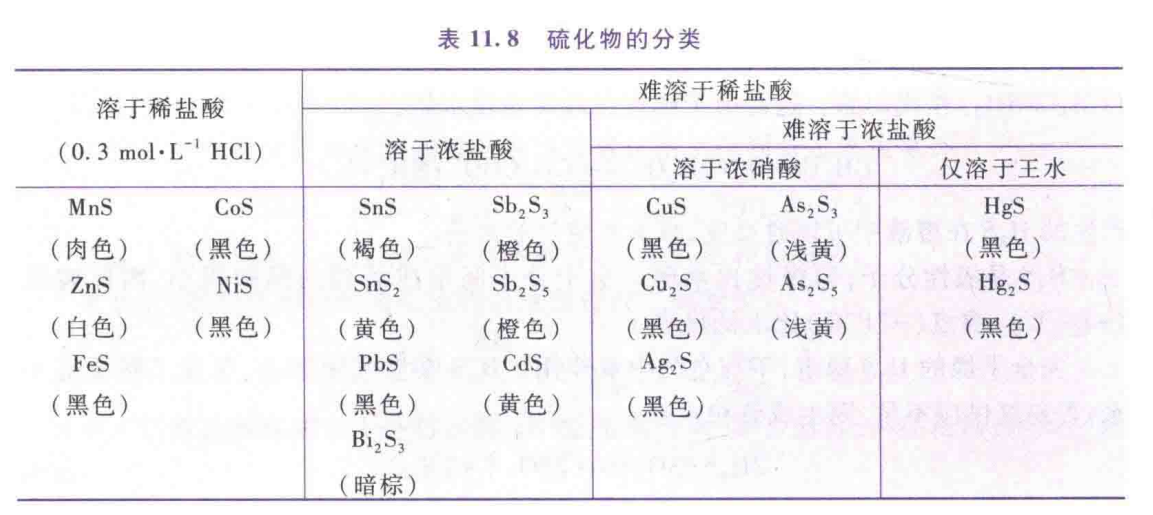
\includegraphics[width=0.8\textwidth]{figure//硫化物分类.png}
	\caption{硫化物的分类}
	\label{fig:}
\end{figure}

随着\ce{K_{sp}}从高到低,\ce{MS}型硫化物具有以下分类:

(1)难溶于水,溶稀盐酸,如\ce{ZnS}

(2)难溶于水和稀盐酸,溶于浓盐酸(这是因为生成配合物使得反应正向移动),如\ce{PbS}

(3)难溶于水和盐酸,但溶于浓硝酸(这是因为发生氧化还原反应)

(4)仅溶于王水(因为王水既能氧化\ce{S^2-},也能拆出金属阳离子形成配合物)\\

\ce{Na2S}水解呈碱性,俗称“硫化碱”,有时代替\ce{NaOH}使用。\\

3.多硫化物

在可溶性硫化物的浓溶液中加入硫粉便可生成相应的多硫化物。

$$ \ce{Na2S + (x-1)S -> Na2S_x}(x = 2\sim 6) $$

随着硫原子数(x)的增加,多硫化物颜色从黄色变为橙黄变为红色。

多硫化物与过氧化物相似,具有氧化型和还原性,在酸性中很不稳定容易歧化为单质硫和硫化氢。所以,碱性多硫化物如\ce{(NH4)2S2}可溶解一些非金属硫化物,如\ce{As,Sb}。在碱性环境中二硫化钠(\ce{Na2S2})氧化硫化亚砷(\ce{As2S3}):

$$ \ce{As2S3 + 2Na2S2 -> As2S5(\text{棕黄色}) + 2Na2S} $$

在酸性环境中\ce{(NH4)2S2}氧化硫化砷:

$$ \ce{As2S3 + (NH4)2S2 -> (NH4)3AsS4 + S v } $$

除此之外,多硫化物的氧化性也可以氧化一些金属硫化物,如\ce{Sn}:

$$ \ce{Na2S2 + SnS -> Na2[SnS3]} $$

而\ce{Na2S}是不能与\ce{SnS}反应的,因为本质上是\ce{Na2S2}将\ce{Sn}从二价氧化为四价,进而发生:

$$ \ce{Na2S + SnS2 -> Na2[SnS3]} $$

这一点可以用于区分\ce{SnS,SnS2}。

\subsubsection{硫的氧化物、含氧酸、盐}

1.硫的氧化物

主要有两种,二氧化硫和三氧化硫。

\ce{SO2}:

物理性质:\ce{SO2}为无色具有强烈刺激性气味的有毒气体,易液化。

氧化/还原性:还原性较显著。

特殊反应:有些有机物能与\ce{SO2}发生加成反应,生成无色加成物。

大气污染:可利用\ce{CO}将\ce{SO2}还原为硫,也可以用石灰乳吸收。

\ce{SO3}:

易挥发的无色固体,有强氧化性,可令单质磷燃烧,将碘化物氧化为单质碘。\\

2.硫的含氧酸及其盐

分为:亚硫酸、硫酸、连硫酸、过硫酸四个系列(见P278)。\\

(1)亚硫酸及其盐:

制备:\ce{SO2}在水中生成亚硫酸\ce{H2SO3},为二元中强酸;向亚硫酸盐加入酸可产生\ce{SO2}。

溶解性:正盐(除\ce{K+,Na+,NH4+})都难溶于水,酸式盐都可溶于水。

热稳定性:亚硫酸盐受热易分解为硫酸盐和硫化物。\\

(2)硫酸及其盐

\textbf{硫酸}:\\

制备:工业上用接触法,在空气中焙烧黄铁矿或硫磺制得\ce{SO2},再通过催化剂氧化为\ce{SO3},再用浓硫酸吸收即可制得发烟硫酸。

结构:中心S原子进行$sp^3$杂化,形成4个$\sigma$键,非羟基氧的2p电子与\ce{S}的3d电子形成$(p-d)\pi 键$,这两个氧原子可近似看做与中心S原子形成双键。(P280)

含氧酸根\ce{ClO4-,PO4^3-,SIO4^4-}结构都类似。

物理性质:纯硫酸是无色油状液体,沸点高、难挥发,可以利用这一点制备挥发性的硝酸和盐酸。

酸性:二元酸中酸性最强的,第二步解离中\ce{HSO4-}相当于中强电解质。

稳定性:较稳定,沸点以上可分解为\ce{SO3}和水。

吸水性:浓硫酸与水混合,形成水合物放出大量热;还可夺取有机化合物中比例为2:1的氢和氧,令有机物碳化。

氧化性:热、浓\ce{H2SO4}氧化型较强,与金属(如\ce{Cu})与非金属(如\ce{C})反应时一般被还原为\ce{SO2}。

由于\ce{Zn}的强还原性,浓硫酸与之反应时还会被还原为硫单质和硫化氢。

\ce{Al,Fe,Cr}在冷、浓\ce{H2SO4}中被钝化。\\

\textbf{硫酸盐和矾}:\\

溶解性:酸式硫酸盐中大部分易溶于水;硫酸盐中除了\ce{Ba,Pb,Ca,Sr}盐难溶,\ce{Ag2SO4}稍溶,其余都易溶。

矾:带结晶水的过渡金属硫酸盐,例如五水合硫酸铜称为胆矾和蓝矾。但严格的说,矾应当符合以下通式:

$$ \ce{M(I)2SO4 * M(II)SO4 * 6H2O} or \ce{M(I)2SO4 * M(III)2(SO4)3 * 24H2O}$$

严格符合上述通式的有莫尔盐(\ce{NH4+,Fe^2+})、明矾(\ce{K+,Al^3+})。

热稳定性:活泼金属硫酸盐在高温下稳定,重金属的硫酸盐则会分解为金属氧化物或单质。

$$ \ce{CuSO4 ->[\Delta] CuO + SO3 ^} $$

$$ \ce{2Ag2SO4 ->[\Delta] 4Ag + 2SO3 ^ + O2 ^} $$

(3)焦硫酸及其盐

物理性质:无色晶状固体,熔点$35^\circ C$。

制备:等物质量的三氧化硫和纯硫酸化合:

$$ \ce{SO3 + H2SO4 -> H2S2O7} $$

或者酸式硫酸盐加热脱去\ce{SO3}:

$$ \ce{2KHSO4 ->[\Delta] K2S2O7 + H2O} $$

进一步加热,再脱去\ce{SO3}则又生成硫酸盐。

焦硫酸可看作是两分子硫酸脱去一分子水的产物。反过来,焦硫酸与水反应可生成硫酸。

化学性质:比硫酸具有更强的氧化性、吸水性、腐蚀性,是良好的磺化剂。

用途:可作熔矿剂,与矿物共熔生成可溶的金属硫酸盐。

(4)硫代硫酸及其盐:

制备:将硫粉溶于沸腾的亚硫酸钠中即可制得,俗称为海波或大苏打:

$$ \ce{Na2SO3 + S -> Na2S2O3} $$

可看作是\ce{SO4^2-}的一个氧原子被硫原子取代。

物理性质:无色透明晶体,易溶于水,水溶液呈弱碱性。

稳定性:\ce{S2O3^2-}在酸性溶液不稳定,易分解为单质硫和二氧化硫(生成黄色沉淀和刺激性气体):

$$ \ce{S2O3^2- + H+ -> S v + SO2 ^ + H2O} $$

重金属的硫代硫酸盐也不稳定,\ce{Ag2S2O3}在溶液中迅速分解,颜色经黄色、棕色,最后为黑色\ce{Ag2S}。

$$ \ce{Ag2S2O3 + H2O -> Ag2S v + H2SO4} $$

氧化性:中强还原剂,与强氧化剂反应被氧化为硫酸钠,被弱氧化剂(如碘)氧化为连四硫酸钠,后者被用于定量测定碘。

$$ \ce{2S2O3^2- + I2 -> S4O6^2- + 2I-} $$

配位性:\ce{S2O3^2-}是较强配体,可与多种重金属形成配合物,如\ce{[Ag(S2O3)2]^3-}。

鉴定:见稳定性。\\

(5)过硫酸及其盐:

过硫酸:硫的含氧酸中含有过氧基的称为过硫酸。过硫酸可视为过氧化氢的衍生物。

物理性质:过二硫酸是无色晶体,有强吸水性,能使有机物碳化。

化学性质:过二硫酸不稳定,容易水解生成硫酸和过氧化氢。

$$ \ce{H2S2O8 + H2O -> H2SO4 + H2SO5} $$

$$ \ce{H2SO5 + H2O -> H2SO4 + H2O2} $$

氧化性:过硫酸盐是强氧化剂,在\ce{Ag+}催化下可氧化\ce{Mn^2+}为\ce{MnO4-}。

稳定性:不稳定,受热易分解为硫酸根、三氧化硫和氧气。\\

(6)连二亚硫酸钠:

物理性质:白色粉末状固体,俗称保险粉,可溶于冷水。

制备:锌粉还原亚硫酸氢钠:

$$ \ce{2NaHSO3 + Zn -> Na2S2O4 + Zn(OH)2} $$

稳定性:水溶液不稳定,容易分解为硫代硫酸根:

$$ \ce{2Na2S2O4 ->[\Delta] Na2SO3 + SO2 ^ + Na2S2O3} $$

还原性:很强,可还原碘、碘酸盐、氧气、银离子、铜离子等:

$$ \ce{Na2S2O4 + O2 + H2O -> NaHSO3 + NaHSO4} $$

此反应可用于分析氧气。

\section{氮族、碳族和硼族}

\subsection{氮族元素}

\subsubsection{概述}

氮族元素:周期表中第VA族的氮、磷、砷、锑、铋、鏌。

价层电子构型为$ns^2np^3$,容易形成正氧化数化合物。

存在惰性电子对效应,从上到下氧化数为+3的物质稳定性增加,氧化数为+5的物质稳定性降低(IIIA,IVA祖业存在此现象)。

与其他元素结合主要通过共价键,且氮族元素原子越小,形成共价键的趋势越大。但活泼金属的氮化物和磷化物是离子型的,如\ce{Mg3N2,Ca3P2}。

\subsubsection{氮气}

1.制备:

实验室中加热分解亚硝酸氨:

$$ \ce{NH4NO2 -> N2 ^ + 2H2O} $$

工业上采用液态空气分馏。\\

2.氮气的稳定性和等电子体

氮气中两个氮原子以叁键结合,键能大,常温下很稳定。

等电子体:具有相同电子数和原子数的分子,等电子体具有相似的结构和类似的性质。

例如,\ce{N2}和\ce{CO}为等电子体。

\subsubsection{氨及铵盐}

1.氨

制备:工业上采用高温高压下,氮气和氢气化合;实验室上则用铵盐和碱反应。

物理性质:无色,有刺激性臭味的气体;是一种良好溶剂,能溶解碱金属和碱土金属。

化学性质:氨能发生如下三类反应:\\

(1)加合反应。因为\ce{N}原子上有孤电子对,容易发生加合反应,例如形成\ce{NH3 * H2O},\ce{2NH3 * H2O}。

除此之外,氨还可以与金属离子和一些分子加和:

$$ \ce{NH3 + H+ -> NH4+} $$

$$ \ce{Cu^2+ + 4NH3 -> [Cu(NH3)4]^2+} $$

$$ \ce{CaCl2 + 8NH3 -> CaCl2 * 8NH3} $$

(2)取代反应。氨分子中的氢原子可依次被取代,生成氨基化物(\ce{-NH2})、亚氨基化物(\ce{=NH})、氮化物(\ce{#N});另一种形式是氨基取代其他化合物中的原子或原子团,如:

$$ \ce{HgCl2 + 2NH3 -> Hg(NH2)Cl v + NH4Cl} $$

(3)氧化反应。根据反应温度的不同,氨与氧反应可生成氮气或一氧化氮;也可与某些氧化物反应:

$$ \ce{3CuO + 2NH3 ->[\Delta] 3Cu + N2 ^ + 3H2O} $$

也可以与\ce{Cl2,Br2}反应:

$$ \ce{3Cl2 + 2NH3 -> N2 ^ + 6HCl} $$

工业上用此检查氯气管道是否漏气。\\

2.铵盐

铵盐的离子半径、电荷数与\ce{K+}很接近,故铵盐在晶型、颜色、溶解度都与相应钾盐类似。

颜色:一般无色,有色按照阴离子颜色。

鉴定:在铵盐溶液中加入强碱释放氨。

$$ \ce{NH4+ + OH- -> NH3 ^ + H2O} $$

热稳定性:固态铵盐加热记忆分解,分解产物与阴离子和分解温度有关。

对于非氧化性的酸盐,逸出氨:

$$ \ce{NH4Cl ->[\Delta] NH3 ^ + HCl ^ } $$

对于氧化型的铵盐,分解为\ce{N2}或氮的氧化物:

$$ \ce{NH4NO2 ->[\Delta] N2 ^ + 2H2O} $$

$$ \ce{NH4NO3 ->[\sim 210^\circ C] N2O ^ + 2H2O} $$

$$ \ce{2NH4NO3 ->[higher than 300^\circ C] 2N2 ^ + O2 ^ + 4H2O ^} $$

$$ \ce{(NH4)2Cr2O7 ->[\Delta] N2 ^ + Cr2O3 + 4H2O} $$

\subsubsection{氮的氧化物、含氧酸及其盐}

1.氮的氧化物

氮从+1到+5均可形成氧化物,\ce{NO}液态和固态为蓝色,\ce{N2O3}为蓝色液体(容易分解为\ce{NO2,NO}),\ce{NO2}为红棕色气体(具有强氧化性),\ce{N2O4}为无色气体(分解为\ce{NO2}),其余均无色,\ce{N2O5}不稳定。\\

2.氮的含氧酸及其盐

(1)亚硝酸及其盐。

亚硝酸:

制备:\ce{NO},\ce{NO2}等物质量溶解在水中,or向亚硝酸盐溶液加入硫酸:

$$ \ce{NO + NO2 + H2O ->[\text{冷}] 2HNO2} $$

热稳定性:亚硝酸不稳定,溶液浓缩或加热时分解为\ce{N2O3},再分解为\ce{NO,NO2}。

$$ \ce{2HNO2 <=> N2O3(\text{蓝色}) + H2O <=> NO2(\text{红棕色}) ^ + NO ^ + H2O} $$

亚硝酸盐:

鉴定:亚硝酸盐遇到强酸生成\ce{HNO2},\ce{HNO2}按照上式分解,先令水溶液呈蓝色,再产生红棕色气体。

热稳定性:亚硝酸盐热稳定性较高。

制备:金属高温下还原固态硝酸盐,如:

$$ \ce{Pb + KNO3 -> PbO + KNO2} $$

尾气处理:用碱液吸收\ce{NO,NO2}尾气,得到亚硝酸钠。

溶解性:一般易溶于水,但黄色\ce{AgNO2}难溶。

氧化/还原性:酸性溶液中是强氧化剂,本身被还原为\ce{NO};与强氧化剂反应被氧化为\ce{NO3-}。

配位性:氮和氧原子上都有孤对,所以它是一种很好的配体,形成如\ce{[Co(NO2)6]^3-}。\\

(2)硝酸及其盐

\textbf{硝酸}

制备:工业上采用氨催化氧化法,先将氨氧化为\ce{NO},再氧化为\ce{NO2},溶于水得到\ce{HNO3}。

结构:\ce{HNO3}中氮原子采用$sp^2$杂化轨道,三个单电子形成三个$\sigma$键,孤电子对不参与杂化,与两个非羟基氧原子的2p轨道上的单电子形成$\Pi_3^4$大$\pi$键;\ce{NO3-}中,大$\pi$键加上一个氧原子的一个单电子和一个外来电子变为$\Pi_4^6$。

物理性质:无色液体,易挥发,能与水任意比例互溶;硝酸常呈黄到棕色,这是因为硝酸受热、见光分解为\ce{NO2}溶于\ce{HNO3}中。

$$ \ce{4HNO3 ->[heat or light] 4NO2 ^ + O2 ^ + 2H2O} $$

酸性:强酸性。

氧化性:强氧化性,非金属元素如\ce{C,P,S,I}等都能被浓硝酸氧化为相应的氧化物或含氧酸,硝酸还原为\ce{NO}:

$$ \ce{3C + 4HNO3 -> 3CO2 ^ + 4NO ^ + 2H2O} $$

$$ \ce{3P + 5HNO3 + 2H2O -> 3H3PO4 + 5NO ^} $$

$$ \ce{S + 2HNO3 -> H2SO4 + 2NO ^} $$

$$ \ce{3I2 + 10HNO3 -> 6HIO3 + 10NO ^ + 2H2O} $$

与金属反应:

\begin{tabular}{c|c|c|c|c}

	金属&\ce{Ca,Ag,Cu}&\ce{Sn,W,Sb}&\ce{Al,Fe,Cr}&\ce{Au,Pt,Rh}\\ \hline
	反应产物&可溶性硝酸盐如\ce{Ca(NO3)2}&难溶氧化物如\ce{SnO2}&钝化&不反应\\

\end{tabular}

\ce{Au,Pt}等贵金属可用王水溶解,因为金属离子可形成稳定配离子,令其电极电势减小,反应向\ce{Au,Pt}溶解的方向进行:

$$ \ce{Au + HNO3 + 4HCl -> H[AuCl4] + NO ^ + 2H2O} $$

硝酸被金属还原程度取决于硝酸浓度和金属活泼性,如:

\begin{tabular}{c|c|c}

	硝酸/金属&活泼金属&不活泼金属\\ \hline
	浓硝酸&NO2&NO2\\
	稀硝酸&N2O&NO\\
	极稀硝酸&NH4NO3&...\\

\end{tabular}

可以看出,硝酸越稀,氮被还原的程度越大。

\begin{tcolorbox}

	为什么稀硝酸被还原的程度大不能说明其氧化性更强?

	首先,一个原子得几个电子不能说明其氧化性的强弱,应该通过电极电势判断。

	$$ \ce{NO3- + 2H+ + e- -> NO2 + H2O} $$

	$$ \ce{NO3- + 4H+ + 3e- -> NO + 2H2O} $$

	根据能斯特方程,

	$$ E = E^\theta + \frac{RT}{zF}lnK $$

	第一,它们的电极电势与\ce{H+},\ce{NO3-}的浓度有关;第二,高价态化合物不一定意味着高电势,如高氯酸的氧化性就大大不如次氯酸,这是因为高氯酸结构更稳定,且有反馈$\pi$键,不容易断键氧化。

	比较$高浓度下E^\Theta(\ce{NO3-/NO2})和低浓度下E^\Theta(\ce{NO3-/NO})$即可得知,浓硝酸氧化性更强。

\end{tcolorbox}

\textbf{硝酸盐}

物理性质:无色、易溶于水的离子晶体,水溶液无氧化性。

热稳定性:常温稳定,受热分解显氧化性。

除了硝酸铵外,硝酸盐受热分解有三种情况:

碱金属和碱土金属(除\ce{Li,Be,Mg})的硝酸盐分解产生亚硝酸盐和氧气:

$$ \ce{2NaNO3 ->[\Delta] 2NaNO2 + O2 ^} $$

活泼性较小的金属(\ce{Mg}与\ce{Cu}之间)硝酸盐热分解得到金属氧化物、\ce{NO2,O2}:

$$ \ce{2Pb(NO3)2 ->[\Delta] 2PbO + NO2 ^ + O2 ^} $$

活泼性更小的金属(比\ce{Cu}小)硝酸盐分解为金属单质、\ce{NO2,O2}。

$$ \ce{2AgNO3 ->[\Delta] 2Ag + 2NO2 ^ + O2 ^} $$

由于以上的性质,硝酸盐与可燃物质混合时会迅速燃烧,可用于制造烟火及黑火药。

鉴定:棕色环实验:向硝酸盐溶液的试管中加入少量硫酸亚铁晶体,小心加入浓硫酸,由于生成棕色配离子,\ce{[Fe(NO)(H2O)5]^2+},浓硫酸和溶液界面处出现棕色环:

$$ \ce{3Fe^2+ + NO3- + 4H+ -> 3Fe^3+ + NO +2H2O} $$

$$ \ce{[Fe(H2O)6]^2+ + NO -> [Fe(NO)(H2O)5]^2+(\text{棕色}) + H2O} $$

\ce{NO2-}也有类似反应,但得到的是棕色溶液:醋酸溶液中,\ce{FeSO4}与\ce{NO2-}反应呈棕色。\ce{NO2-}的存在会干扰\ce{NO3-}的鉴定,为排除干扰可加入\ce{NH4Cl}共热,破坏\ce{NO2-}。

\subsubsection{磷的含氧酸及其盐}

磷有多重含氧酸:(P298结构)

\begin{tabular}{c|c|c|c|c|c|c}

	名称&正磷酸&焦磷酸&三聚磷酸&偏磷酸&亚磷酸&次磷酸\\ \hline
	化学式&\ce{H3PO4}&\ce{H4P2O7}&\ce{H5P3O10}&\ce{HPO3}&\ce{H3PO3}&\ce{H3PO2}\\
	氧化数&+5&+5&+5&+5&+3&+1\\
	n元酸&3&4&5&1&2&1\\

\end{tabular}

焦磷酸、三聚磷酸为一个系列,它们分别是两个、三个正磷酸脱水缩合的产物;

亚磷酸、次磷酸为一个系列,它们分别是正磷酸去掉一个、两个非羟基氧的产物;

偏磷酸是正磷酸去掉一个羟基的产物。\\

1.(正)磷酸

结构:集合上,由单一的磷氧四面体构成。与\ce{H2SO4}类似,\ce{H3PO4}中也有$(p-d)\pi 键$。

制备:工业上用硫酸分解磷灰石(磷酸钙)制取磷酸:

$$ \ce{Ca3(PO4)2 + 3H2SO4 -> H3PO4 + 3CaSO4} $$

物理性质:无色透明粘稠液体或晶体。

酸性:三元中强酸。

氧化性:无。

配位性:很强,能与许多金属离子形成配合物,例如\ce{H3[Fe(PO4)2]}、\ce{H[Fe(HPO4)2]}等。

特殊反应:缩合作用,多个磷酸单分子可通过失去水分子连接在一起,多聚磷酸为缩合酸,一般缩合酸的酸性比正酸要强。\\

2.磷酸盐

磷酸盐有三种:磷酸正盐,磷酸一氢盐,磷酸二氢盐。

只要控制pH,\ce{H3PO4}的三种钠盐均可通过与\ce{NaOH}反应获得。

溶解性:磷酸二氢盐均溶于水,其他两种类型除了\ce{K+,Na+,NH4+}一般难溶。

鉴定:在含有硝酸的水溶液中,将\ce{PO4^3-}与过量钼酸铵\ce{(NH4)2MoO4}混合加热,析出黄色磷钼酸铵沉淀:

$$ \ce{PO4^3- + 12MoO4^2- + 24H+ + 3NH4+ -> (NH4)3PO4 * 12MoO3 * 6H2O v (\text{黄色}) + 6H2O} $$

\subsubsection{砷、锑、铋及其重要化合物}

1.砷锑铋单质

价层电子构型为$ns^2np^3$,阳离子为18或18+2电子构型,具有较强极化能力和较大变形性。砷锑具有两性和准金属性质,铋呈金属性。

物理性质:熔点较低,易挥发,气态时以多原子分子形式存在,如\ce{As4,As2,Sb4,Sb2,Bi2}。

制备:煅烧硫化物为氧化物,再还原氧化物。\\

2.砷锑铋的氧化物及其水化物

砷锑铋有+3和+5两个系列的氧化物:

\begin{tabular}{c|c|c|c|c|c}

	\ce{As2O3}&\ce{Sb2O3}&\ce{Bi2O3}&\ce{As2O5}&\ce{Sb2O5}&\ce{Bi2O5}\\ \hline
	白色&白色&黄色&白色&淡红色&红棕色\\

\end{tabular}

\ce{As2O3}为砒霜,剧毒,微溶于水,热水中溶解度较大,溶解生成亚砷酸\ce{H3AsO3};\ce{As2O3}为两性偏酸的化合物,易溶于碱生成亚砷酸盐,溶于浓盐酸生成\ce{As(III)}盐:

$$ \ce{As2O3 + 6NaOH -> 2Na2AsO3 + 3H2O} $$

$$ \ce{As2O3 + 6HCl -> 2AsCl3 + 3H2O} $$

\ce{Sb2O3}具有明显两性,\ce{Bi2O3}为弱碱性,可看出它们氧化物的水化物按照\ce{H3AsO3-Sb(OH)3-Bi(OH)3}的顺序酸性减弱、碱性增强(原因:离子势、酸碱解离)。

氧化数为+5的砷锑铋的氧化物都呈酸性,与水反应可制得砷酸、锑酸但得不到铋酸,需要:

$$ \ce{Bi(NO3)3 + NaClO + 4NaOH -> NaBiO3 v (\text{黄色}) + 3NaNO3 + NaCl + 2H2O} $$

得到铋酸钠。\\

从上到下,三价化合物的还原性减弱,五价化合物氧化性增强。并且,砷酸盐、锑酸盐在强酸性溶液中显出明显氧化性。

\begin{tcolorbox}

	为什么有些离子的氧化性受到pH的影响?
	
	例如\ce{NO3-},\ce{H3AsO4},它们的氧化性与溶液酸度有关。这是因为它们在氧化还原反应中涉及到\ce{O}数目的变化,而这就导致反应中涉及\ce{H+}或\ce{OH-},在能斯特方程中影响$E^\Theta$从而导致氧化性变化。

\end{tcolorbox}

铋酸盐在酸性溶液中氧化性如此之强,以至于可以将\ce{Mn^2+}氧化为\ce{MnO4-}:

$$ \ce{2Mn^2+ + 5NaBiO3 + 14H+ -> 2MnO4- (\text{紫红色}) + 5Bi^3+ + 5Na+ + 7H2O} $$

此反应用来鉴别\ce{Mn^2+}。\\

总结:

\begin{figure}[htpb]
	\centering
	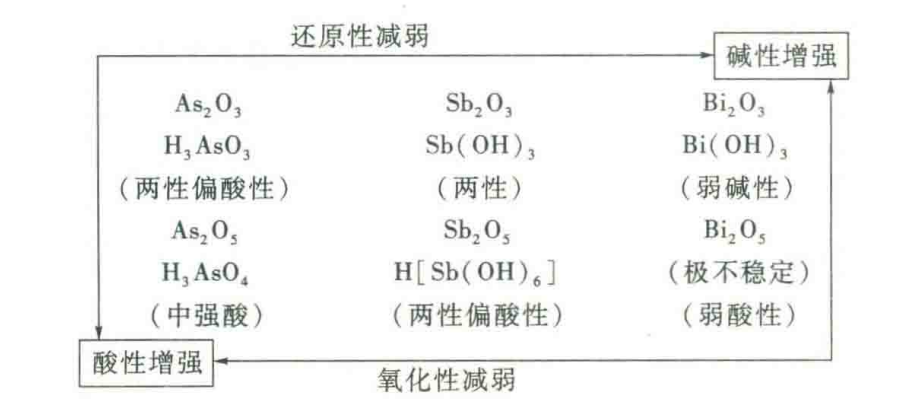
\includegraphics[width=0.8\textwidth]{figure//砷锑铋的变化规律.png}
	\caption{砷锑铋的变化规律}
	\label{fig:}
\end{figure}

3.砷锑铋的盐

有两种:一种阴离子盐(\ce{MO3^3-,MO4^3-},一种阳离子盐(\ce{M^3+,M^5+})。

三价阳离子氯化物极易水解,除\ce{As}外生成白色碱式盐沉淀(如\ce{SbOCl})和\ce{HCl}。

\ce{Sb(III),Bi(III)}的硝酸盐也极易水解,生成碱式盐程度(\ce{SbONO3})和\ce{HNO3}。

无论是阴离子盐还是阳离子盐都可在酸性情况与\ce{H2S}反应,得到有色相应硫化物沉淀:

$$ \ce{2As^3+ + 3H2S -> As2S3 v (\text{淡黄色}) + 6H+} $$

$$ \ce{2AsO3^3- + 3H2S + 6H+ -> As2S3 v + 6H2O} $$

砷的硫化物是黄色的,锑的为橙红色,铋的为黑色;只有\ce{Bi2S3}为碱性且不溶于碱性硫化物(如\ce{Na2S,(NH4)2S}),其余均为两性且溶于碱性硫化物:

$$ \ce{As2S3 + 3S^2- -> 2AsS3^3- (\text{硫代亚砷酸根})} $$

$$ \ce{Sb2S3 + 3S^2- -> 2SbS3^3- (\text{硫代亚锑酸根})} $$

$$ \ce{As2S5 + 3S^2- -> 2AsS4^3- (\text{硫代砷酸根})} $$

$$ \ce{Sb2S5 + 3S^2- -> 2AsS4^3- (\text{硫代锑酸根})} $$

\ce{As2S3}还可溶于\ce{KOH}溶液中:

$$ \ce{As2S3 + 6OH- -> AsS^3- + AsO3^3- + 3H2O} $$

硫代酸盐很不稳定,立即分解为相应的难溶硫化物并放出硫化氢气体:

$$ \ce{2AsS3^3- + 6H+ -> 2H3AsS3 -> As2S3 v + 3H2S ^ } $$

$$ \ce{2AsS4^3- + 6H+ -> 2H3AsS4 -> As2S5 v + 3H2S ^ } $$

\subsection{碳族元素}

\subsubsection{碳族元素概述}

碳族元素:周期系第IV A族元素,包括碳硅锗锡铅和铁六种元素。

碳族元素自上而下为非金属碳硅,到准金属锗,再到金属锡和铅。

价电子构型为$ns^2np^2$,形成+2,+4的化合物。锗和锡的二价化合物具有强还原性,铅(IV)的化合物具有强氧化性。\\

锡疫:当温度在$ -30^\circ C \sim 40^\circ C $时,白锡会迅速转变为粉末状的灰锡。

\subsubsection{碳及其重要化合物}

1.碳的同素异形体

石墨、金刚石、富勒烯碳是碳的主要同素异形体;木炭、炭黑、活性炭、焦炭都是石墨的微晶体。\\

2.碳的氧化物

\ce{CO}是无色无臭有毒的气体,有还原性、加和性,可形成金属羰基化合物如\ce{[Ni(CO)4]}。

\ce{CO2}是无色无臭的气体,易液化,固态称为干冰。\\

3.碳酸及其盐

(1)碳酸

二元弱酸,极不稳定,很弱。\\

(2)碳酸盐

\textbf{溶解性}

除了铵和碱金属(除锂)的碳酸盐之外,多数碳酸盐难溶于水,大多数酸式碳酸盐易溶于水。

对于难溶碳酸盐来说,其相应的酸式盐比正盐的溶解度大(如\ce{CaCO3,Ca(HCO3)2};对于易溶碳酸盐来说,其相应的酸式盐比正盐的溶解度小(如\ce{Na2CO3,NaHCO3})。

\textbf{水解性}

可溶碳酸盐的水溶液呈碱性,酸式碳酸盐水溶液呈微碱性。

纯碱:碳酸钠。

洗涤碱:十水碳酸钠。

金属离子与可溶性碳酸盐可发生沉淀,有三种形式:

若金属氢氧化物溶解度小于相应碳酸盐(如\ce{Al(III),Fe(III),Cr(III)}),生成氢氧化物沉淀。

若金属氢氧化物溶解度相差不大(\ce{Bi(III),Cu(II),Mg(II)}),生成碱式碳酸盐沉淀。

若金属氢氧化物溶解度大于相应碳酸盐(\ce{Ca(II),Sr(II),Ba(II),Ag(I),Cd(II),Mn(II)}),生成碳酸盐沉淀。

\textbf{热稳定性}

金属离子的极化能力越强,碳酸盐的热稳定性越差。


金属碳酸盐中,金属离子只极化附近的一个\ce{O^2-},与\ce{C^4+}产生的偶极方向相反,削弱了碳氧键,所以金属极化力越强,反极化作用越强,碳酸盐越不稳定。

反极化作用:两个离子形成相反方向的电场,相互削弱对方对某离子的影响,称为反极化作用。

热稳定性碳酸盐>碳酸氢盐>碳酸的原因是\ce{H+}强极化作用的影响。

热稳定性的一般规律是:碱金属盐>碱土金属盐>过渡金属盐>铵盐;碳酸盐>碳酸氢盐>碳酸。

\subsubsection{硅及其重要化合物}

1.单质硅

化学性质:硅的化学性质不活泼,室温只与强碱或硝酸和氢氟酸的混合物反应。

$$ \ce{Si + 2NaOH + H2O -> Na2SiO3 + 2H2 ^} $$

$$ \ce{3Si + 4HNO3 + 12HF -> 3SiF4 ^ + 4NO ^ + 8H2O} $$

制备:\ce{C}还原二氧化硅,\ce{Cl2}氧化单质硅,精馏后\ce{H2}还原四氯化硅。\\

2.硅烷

硅烷的数目有限,且不存在不饱和化合物。

\begin{tcolorbox}

	为什么碳可形成不饱和化合物而硅不行?

	原因:硅的原子半径比较长,形成肩并肩$\pi$键比较难。

\end{tcolorbox}

硅烷性质活泼,硅甲烷遇到空气自燃,生成水和二氧化硅。\\

3.卤化物

硅的卤化物都是无色的,常温\ce{SiF4}为气体,\ce{SiBr4,SiBr4}为液体,\ce{SiI4}为固体。

氟化硅的制备:二氧化硅和氢氟酸作用,或用酸+氟化物替换氢氟酸。

\ce{SiF4}与\ce{HF}进一步反应生成氟硅酸:

$$ \ce{2HF + SiF4 -> H2[SiF6]} $$

四氯化硅的制备:直接加热化合,或用碳+二氧化硅替换硅。

\ce{SiCl4}是刺激性无色液体,易水解,生成硅酸和氯化氢。\\

4.二氧化硅

二氧化硅不与酸反应,但可以与氢氟酸反应生成氟化硅;与碱反应生成硅酸钠。\\

5.硅酸或硅胶

硅酸通式:\ce{xSiO2 * yH2O}

多硅酸:x大于等于2的硅酸。

偏硅酸:\ce{H2SiO3 + nSiO2}的系列,常用简式\ce{H2SiO3}代表。

硅酸酸性:二元弱酸。

硅酸制备:盐酸与可溶性硅酸盐直接作用。

硅胶:将硅酸凝胶(多硅酸)中大部分水脱去,得到硅酸干胶(即硅胶)。

变色硅胶:含有氯化钴的硅胶,无水时显蓝色,含水\ce{[Co(H2O)6]^2+}呈粉红色。\\

6.硅酸盐

最简单的是偏硅酸盐和正硅酸盐:

$$ \ce{SiO2 + M2O -> M2SiO3} $$

$$ \ce{SiO2 + 2M2O -> M4SiO4} $$

溶解性:仅碱金属的硅酸盐可溶于水。

颜色:重金属的硅酸盐难溶于水且有颜色:

\begin{tabular}{c|c|c|c|c|c}

	Cu&Co&Mn&Al&Ni&Fe(III)\\ \hline
	蓝绿色&紫色&浅红色&无色透明&翠绿色&棕红色\\

\end{tabular}

“水中花园”:在透明的硅酸钠溶液中加入颜色不同的重金属,生成不同颜色的硅酸盐“树”。

水解性:硅酸的酸性很弱,硅酸钠在水中强烈水解呈碱性,加入\ce{NH4Cl}发射完全水解,生成硅酸沉淀和氨气。

\subsubsection{锡和铅的化合物}

1.锡铅的氧化物和氢氧化物

锡和铅有两类((II)(III))氧化物和相应的氢氧化物,酸碱性递变规律见:

\begin{figure}[htpb]
	\centering
	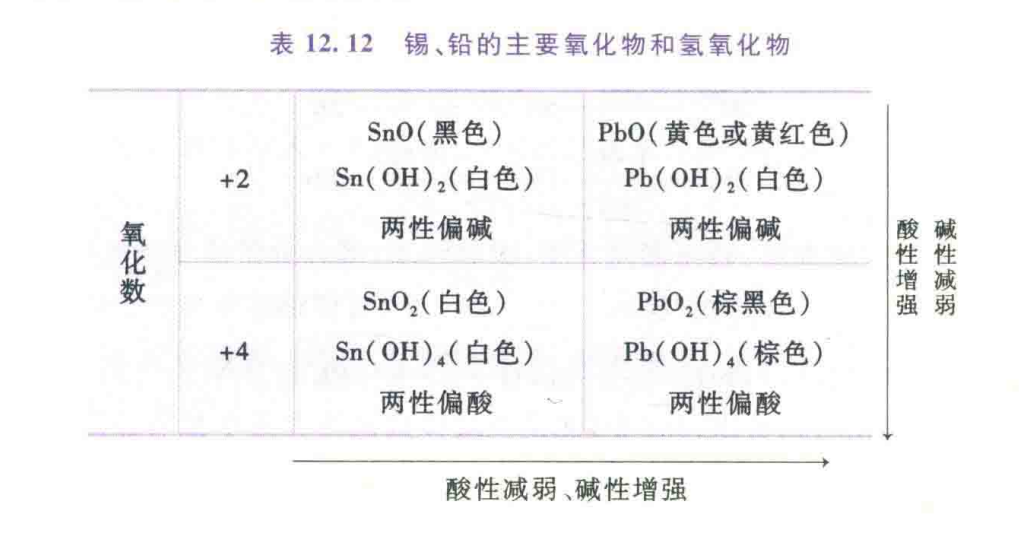
\includegraphics[width=0.8\textwidth]{figure//锡和铅的酸碱性.png}
	\caption{锡和铅的酸碱性}
	\label{fig:}
\end{figure}

铅的氧化物有:\ce{PbO,PbO2}和介于两者之间的鲜红色\ce{Pb3O4},橙色\ce{Pb2O3};有意思的是,它们可以看做是铅酸的铅盐(\ce{Pb2[PbO4]})或铅的不同价态的混合氧化物(\ce{PbO * PbO2})。

\ce{Pb3O4}与稀硝酸反应:

$$ \ce{Pb3O4 + 4HNO3 -> 2Pb(NO3)2 + PbO2 v + 2H2O} $$

可看做\ce{PbO}与酸反应,留下酸性不溶\ce{PbO2}。

同样地,\ce{Pb2O3}与稀硝酸反应有:

$$ \ce{Pb2O3 + 2HNO3 -> Pb(NO3)2 + PbO2 v + H2O} $$

可见\ce{Pb3O4,Pb2O3}的铅具有两种不同的氧化数。\\

\ce{Sn(OH)2,Pb(OH)2}是两性氢氧化物,与碱反应分别生成四羟基合锡、铅。

在\ce{Sn(IV)}化合物溶液中,加入碱金属氢氧化物,生成白色胶状正锡酸\ce{Sn(OH)4},后者容易是转变为偏锡酸,偏锡酸则分为两种。\\

2.锡和铅的盐类

(1)锡(II)的还原性和铅(IV)的氧化性。由于惰性电子对效应,锡的高氧化数状态较稳定,因此\ce{Sn(II)}显还原性;铅的低氧化数状态较稳定,所以\ce{Pb(IV)}显氧化性。

\ce{Sn(II)}在酸碱中均有还原性,且在碱性介质中\ce{[Sn(OH)4]^2-}的还原性更强:

$$ \ce{2Bi^3+ + 6OH- + 3[Sn(OH)4]^2- -> 2Bi v (\text{黑色}) + 3[Sn(OH)6]^2-} $$

这是鉴定\ce{Bi^3+}的一种方法。

\ce{SnCl2}是重要的还原剂,能将汞盐还原成白色亚汞盐:

$$ \ce{2HgCl2 + SnCl2 -> Hg2Cl2 v (\text{白色}) + SnCl4} $$

这是鉴定\ce{Sn^2+}的方法。如果\ce{SnCl2}过量,还可以将亚汞盐还原为黑色金属汞。\\

\ce{PbO2}在酸性中是强氧化剂,可把\ce{Cl-}氧化为氯气,把\ce{Mn^2+}氧化为紫色\ce{MnO4-},与浓硫酸作用放出\ce{O2}:

$$ \ce{PbO2 + 4HCl(\text{浓}) -> PbCl2 + 2Cl2 ^ + 2H2O} $$

$$ \ce{2PbO2 + 2H2SO4(\text{浓}) -> 2PbSO4 + O2 ^ + 2H2O} $$

工业上使用铅蓄电池:

$$ \ce{PbO2 + Pb + 2H2SO4 <=>[\text{放电}][\text{充电] 2PbSO4 + 2H2O}} $$

(2)锡和铅盐的水解性

锡(II)盐和含氧酸盐均易水解生成碱式盐和氢氧化锡沉淀:

$$ \ce{Sn^2+ + Cl- + H2O -> Sn(OH)Cl v + H+} $$

$$ \ce{SnO2^2- + 2H2O -> Sn(OH)2 v + 2OH-} $$

\ce{Sn^2+}盐在空气中容易被氧化为\ce{Sn^4+};\ce{SnCl4}是典型共价化合物,剧烈水解。

\ce{Pb(II)}水解不显著,\ce{PbCl4}为黄色液体,极不稳定,常温分解为\ce{PbCl2}和\ce{Cl2}:

$$ \ce{PbCl4 -> PbCl2 + Cl2 ^} $$

(3)铅盐的难溶性

大多数铅盐难溶于水,卤化铅中\ce{PbI2}为金黄色,溶解度最小,但能生成配合物溶解于\ce{KI}溶液中:

$$ \ce{PbI2 + 2KI -> K2[PbI4]} $$

\ce{PbCl2}难溶于冷水,浓盐酸中形成配合物溶解:

$$ \ce{PbCl2 + 2HCl(\text{浓}) -> H2[PbCl4]} $$

\ce{PbSO4}难溶于水,易溶于浓硫酸(生成酸式盐);在饱和\ce{NH4OAc}溶液中生成铅糖而溶解。

$$ \ce{PbSO4 + 2OAc- -> Pb(OAc)2 + SO4^2-} $$

硝酸铅易水解,加入碳酸钠得到碱式碳酸铅,是一种白色颜料(铅白):

$$ \ce{2Pb^2+ + 2CO3^2- + H2O -> Pb2(OH)2CO3 v + CO2 ^} $$

$\Delta$\ce{Pb^2+}与\ce{CrO4^2-}反应生成黄色铬酸铅沉淀:

$$ \ce{Pb^2+ + CrO4^2- -> PbCrO4 v (\text{黄色})} $$

这一反应用来鉴定\ce{Pb^2+}或\ce{CrO4^2-}。铬酸铅溶于过量碱生成四羟基合铅离子。\\

3.锡和铅的硫化物

锡和铅能形成\ce{MS,MS2}两类硫化物。将硫化氢作用于相应的盐溶液可得到硫化物沉淀(除了\ce{PbS2}不存在)。

它们有如下表:

\begin{tabular}{c|c|c}
	
	\ce{SnS}&\ce{SnS2}&\ce{PbS}\\ \hline
	棕色&黄色&黑色\\
	酸性&酸性&碱性\\

\end{tabular}

\ce{SnS2}与\ce{S^2-}反应,生成硫代锡酸盐(\ce{SnS3^2-})而溶解;\ce{SnS}溶于多硫化铵直接生成硫代锡酸盐。

$$ \ce{SnS2 + S^2- -> SnS3^2-} $$

硫代锡酸盐不稳定,遇酸分解为\ce{SnS2,H2S}。

\ce{PbS}不溶于非氧化性稀酸和碱金属硫化物,但溶于稀硝酸和浓盐酸(硫被氧化、铅形成配合物)。

\subsection{硼族元素}

\subsubsection{概述}

硼族元素:周期系第III A族元素,包括硼铝镓铟铊鉺六种元素。自然界没有游离态的硼。

硼族元素中,除了硼其余均为金属元素,价层电子构型为$ns^2np^1$,常见氧化数为+3,硼铝一般只形成氧化数为+3的化合物。从镓到铊,由于惰性电子对效应,氧化数为+1的化合物更稳定。

硼的原子半径小,电负性大,化合物属于共价型;价电子数为3,轨道数为4,是缺电子原子,可形成缺电子化合物,易形成聚合分子(\ce{Al2Cl6})和配合物(\ce{H[BF4]})。

\subsubsection{硼的氢化物}

物理性质与烷烃、硅烷类似,硼的氢化物称为硼烷,有两种通式:\ce{B_nH_{n+4}}和\ce{B_nH_{n+6}}最简单的是乙硼烷。\\

1.乙硼烷的结构

\ce{B2H6}中,\ce{B}采用不等性$sp^3$杂化,每个\ce{B}原子的4个$sp^3$轨道中有两个连接\ce{H},两个(一个有电子,一个和没有)与另一侧的\ce{B}和一个\ce{H}形成一个三中心二电子的氢桥键,简写为3c-2e。

3c-2e:三中心二电子键(简称三中心键)的简称。

氢桥键:两个硼原子的$sp^3$杂化轨道与两个\ce{H}原子的s轨道形成两个特殊的化学键,犹如通过两个氢原子作为桥梁连接起来,这样的键称为氢桥键。

多中心键:3个或3个以上原子结合形成的共价键,是一种非定域键。多中心键是缺电子原子的一种特殊成键形式,普遍存在于硼烷中。三中心键的强度只有一般共价键的一般,故硼烷的化学性质比烷烃活泼。\\

2.硼烷的性质

物理性质:\ce{B}数的4.5、10.5是气液、液固的分界线;随着原子数目增加,分子变形性增大,熔沸点升高。

热稳定性:乙硼烷在空气自燃,生成氧化硼和水。

水解性:硼烷与水水解为硼酸和氢气,放热。

配位性:能与\ce{NH3,CO}加和,形成配位数为1的配合物。

\subsubsection{硼酸及其盐}

1.(正)硼酸

硼酸的含氧酸包括正硼酸,偏硼酸,多硼酸。正硼酸脱水生成偏硼酸,进一步脱水生成硼酐,此反应可逆。

$$ \ce{H3BO3 <=>[\Delta][H2O] HBO2 <=>[\Delta][H2O] B2O3} $$

硼酸的晶体结构单位\ce{B(OH)3}为平面三角形,具有片状结构,每个硼原子进行$sp^2$杂化,层间借助微弱范德华力联系。

硼酸是一元弱酸,在水中与\ce{OH-}加合形成\ce{[B(OH)4]-}显酸性:

$$ \ce{H3BO3 + H2O <=> [B(OH)4]- + H+} $$

2.硼酸盐

硼砂:四硼酸钠,化学式为\ce{Na2B4O5(OH)4 * 8H2O}或\ce{NaB4O7 * 10H2O},无色透明晶体,容易失水。

铁钴镍锰等金属氧化物,可溶解在硼砂熔体中,显示特征颜色:

$$ \ce{Na2B4O7 + CoO -> Co(BO2)2 * 2NaBO2(\text{蓝色})} $$

$$ \ce{Na2B4O7 + MnO -> Mn(BO2)2 * 2NaBO2(\text{绿色})} $$

硼砂在水中溶解度很大,水解呈碱性:

$$ \ce{B4O7^2- + 7H2O <=> 4H3BO3 + 2OH-} $$

\subsubsection{氧化铝和氢氧化铝}

1.氧化铝

分为\ce{\alpha -Al2O3}和\ce{\gamma -Al2O3}。刚玉属于前者,硬度高;后者可用于作吸附剂和催化剂。\\

2.氢氧化铝

制备:在铝酸盐中通入\ce{CO2},得到氢氧化铝沉淀。

两性:碱性略强于酸性。

\subsubsection{铝盐}

1.三氯化铝

\ce{AlX3}中,\ce{AlF3}为离子化合物,其余的均为共价化合物。

制备:铝盐容易水解,所以制备只能用干法:用\ce{Cl2}氧化金属铝或用\ce{C}和\ce{Al2O3}替代金属铝。

结构:\ce{Al}是缺电子原子,存在空轨道,\ce{Cl}原子有孤电子对,可生成桥式结构的双聚分子\ce{Al2Cl6}。每个\ce{Al}原子以不等性$sp^3$杂化形成4个$\sigma$键和2个3c-4e键,如图:

\begin{figure}[htpb]
	\centering
	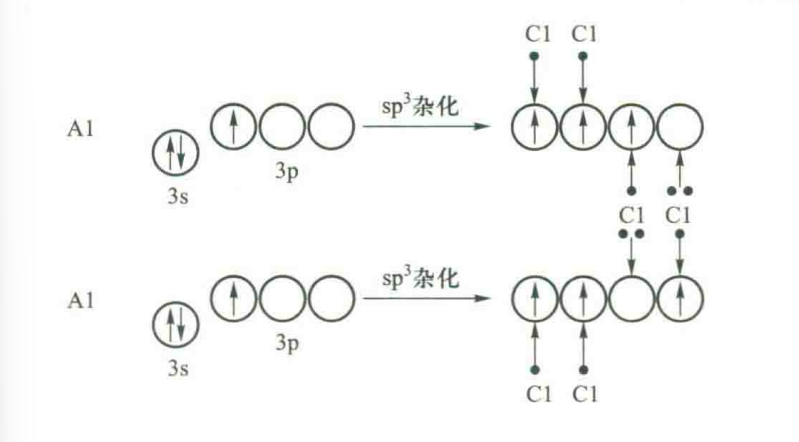
\includegraphics[width=0.5\textwidth]{figure//AlCl3的结构.png}
	\caption{三氯化铝的结构}
	\label{fig:}
\end{figure}

2.硫酸铝

硫酸铝溶液由于\ce{Al^3+}的水解呈酸性,且\ce{Al^3+}实际上以\ce{[Al(H2O)6]^3+}的形式存在:

$$ \ce{[Al(H2O)6]^3+ + H2O <=> [Al(OH)(H2O)5]^2+ + H3O+} $$

进一步水解为\ce{Al(OH)3(H2O)3}。实际书写时,以上的所有水配体都可略去。

有些弱酸会与\ce{Al^3+}相互促进水解,导致完全水解,如\ce{S^2-,CO^2-}。

\subsection{对角关系}

见P322。

\section{过渡元素(一)}

\subsection{概述}

如图:

\begin{figure}[htpb]
	\centering
	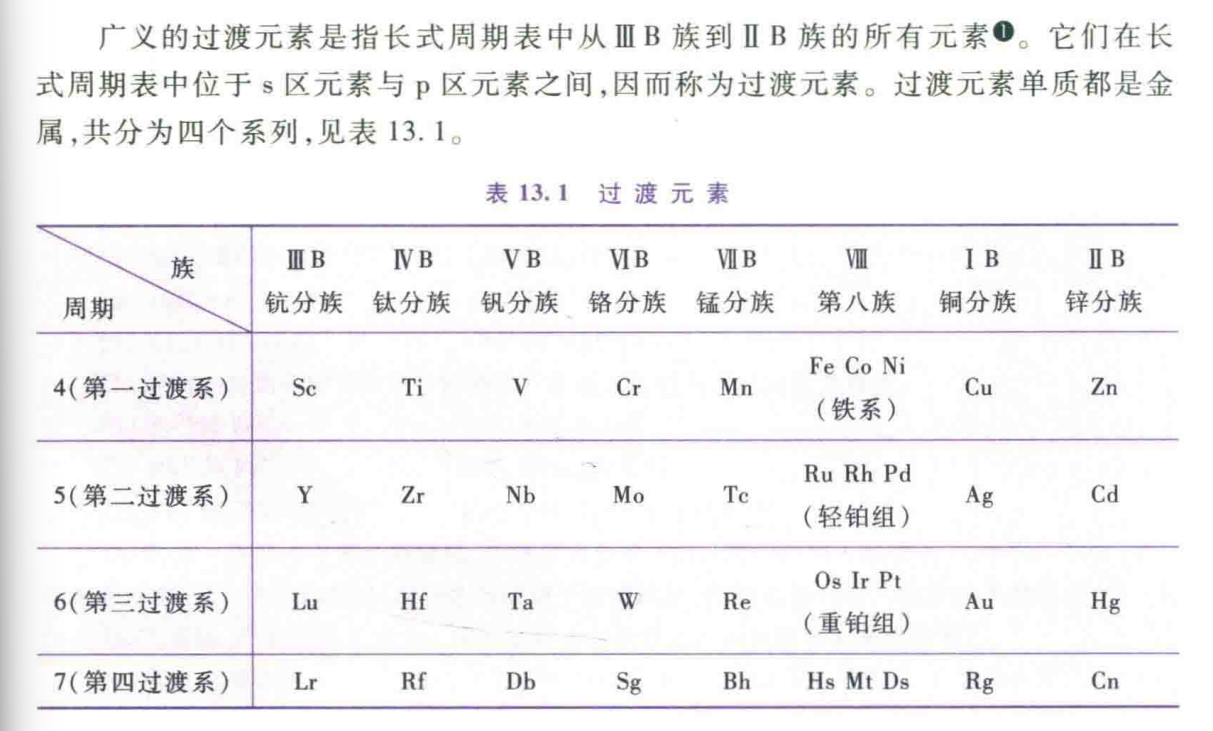
\includegraphics[width=0.8\textwidth]{figure//过渡元素.png}
	\caption{过渡元素分类}
	\label{fig:}
\end{figure}

\subsection{过渡元素原子的特征}

过渡元素原子的特征是价电子一般分布在次外层d轨道,最外s只有1到2个电子。由于类似镧系收缩效应的原因,过渡金属各周期从左向右原子半径缓慢减小,在\ce{Cu}前后又稍增大;同时第二、第三过渡系的同族元素在性质上的差异比第一、第二过渡系相应的元素小。

\subsection{单质的物理性质}

外观多呈银白色或灰白色,有金属光泽;

除了钪钛属于轻金属,其余均属重金属;

熔沸点高、硬度大,熔沸点最高的是钨,硬度最大的是铬;

原因一般认为与 过渡元素原子半径较小而彼此堆积紧密;部分未成对d轨道电子参与成键导致金属键之外还有部分共价性有关。

\subsection{金属活泼性}

过渡金属在水溶液中的活泼性通过$E_A^\Theta$判断。同一周期元素从左向右过渡,总的变化趋势是$E^\Theta(M^{2+}/M)$值逐渐变大,活泼性逐渐减弱。第一周期中,只有\ce{Cu}的标准电极电势是负值,不能置换出氢。

钪分族的钪、钇、镧是过渡元素中最活泼的金属,接近于碱土金属。除了钪分族外,d区同族从上到下活泼性逐渐降低;这是因为同族元素从上到下原子半径增加不多,但有效核电荷数增加多,导致电离能、升华焓增加,金属活泼性减弱。

\begin{tcolorbox}
	
	为什么副族元素同族原子半径相差不大?\\

	这是因为相比主族元素,副族元素有效核电荷数的增加抑制了电子云向外扩张。

	副族元素同族有效核电荷数增加的原因则是由于随着周期数增加,d轨道的电子云形状向外扩散的形状越来越分散,屏蔽效应减弱,对外层电子云的吸引力增强,即有效核电荷数增加。

\end{tcolorbox}
	
第二、三过渡系元素的金属单质非常稳定,不易与强酸反应,但和强碱可反应。

第一过渡系中相邻元素活泼性的相似性超过同族元素。

\subsubsection{氧化数}

过渡元素具有多种氧化数(因为d层也可参与成键)。

1.同周期从左到右变化趋势

其中主要氧化数见下图:

\begin{figure}[htpb]
	\centering
	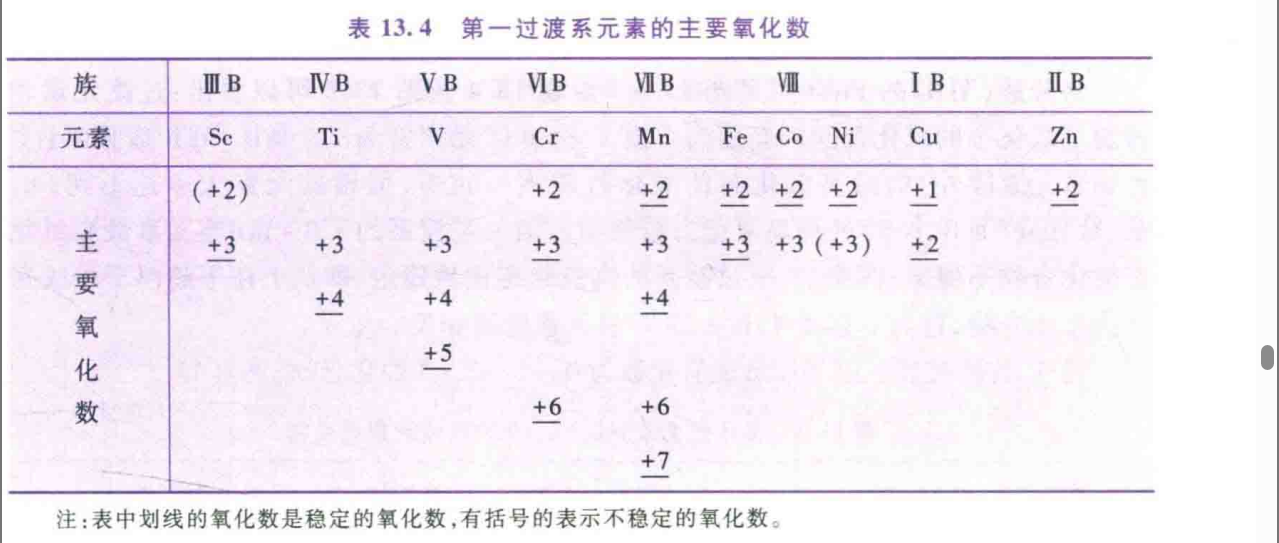
\includegraphics[width=0.8\textwidth]{figure//主要氧化数.png}
	\caption{第一过渡系的主要氧化数}
	\label{fig:}
\end{figure}

值得注意的是,元素最高氧化数先升高再降低,以3d轨道半充满为分界线。\\

2.同族从上到下变化趋势

第一过渡系的VB - VIIB族元素最高氧化态化合物不稳定,二、三的则比较稳定。这与p区恰好相反。

\subsubsection{非整比化合物}

P333

\subsubsection{化合物颜色}

过渡元素形成的配离子大多显色,这与过渡元素离子的d轨道未填满有关,如图:

\begin{figure}[htpb]
	\centering
	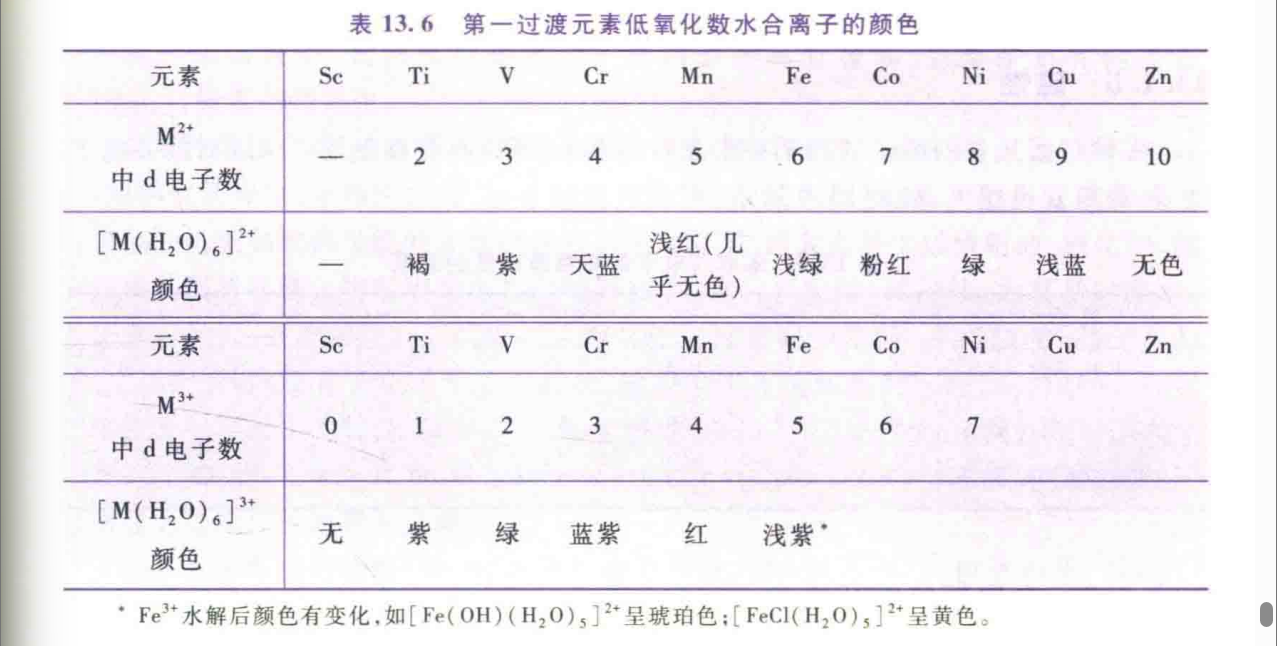
\includegraphics[width=0.8\textwidth]{figure//过渡金属化合物颜色.png}
	\caption{过渡金属水合离子颜色}
	\label{fig:}
\end{figure}

\begin{tcolorbox}
	
	为什么同一中心离子与不同配体形成配合物时颜色不同?\\

	这是因为晶体场分裂能不同,d-d跃迁时需要的能量也不同,即吸收光的波长不同,因此显不同蓝色;

	$d^0和d^{10}$构型的中心离子形成的配合物不会发生d-d跃迁,显示无色;但有些$d^0$构型的如\ce{MnO4-}有颜色是因为电荷迁移导致的(如\ce{MnO4-}的紫色由于氧和锰离子之间的p-d跃迁)。

\end{tcolorbox}

\subsubsection{配合物}

过渡金属容易形成配合物,这是因为过渡金属离子通常具有较高电荷,且属9-17电子构型,极化力和变形性都很强;属于同一能级组的空轨道多,容易形成杂化轨道,有的还能形成$d-p反馈\pi 键$,容易吸引配体。

\begin{tcolorbox}
	
	一个离子的极化力强意味着什么?\\

	一个离子的极化力强,这意味着它更容易令异号电荷离子产生偶极,使离子电子云发生变形,部分重叠,总偶极矩减小。这就是说,它更容易形成共价键,或令键的共价成分更高,所以会导致如下的性质改变:

	1.水中溶解度降低:极化作用令分子极性降低,在极性溶剂中溶解度降低。

	2.物质颜色加深:阴阳离子原子轨道由于重叠能量差减小,电子跃迁吸收可见光能量减小,化合物颜色加深。

	3.晶格类型变化:极化作用令离子键过渡为共价键。

	4.熔沸点降低:同3。

	5.对含氧酸盐热解的影响:酸根中心离子极化能力越强,酸根离子越稳定;金属离子极化作用越强,电荷越高、半径越小(即吸引力越大),越容易夺取\ce{O}原子,热稳定性越差。

	6.对配合物形成的影响:中心离子对配体的极化作用对配体的电子云具有吸引和变形作用,极化作用强让配体更容易被中心离子捕获。

\end{tcolorbox}

\subsubsection{磁性}

大多数过渡元素原子或离子具有未成对电子,具有顺磁性。未成对d电子越多,磁矩越大。

\subsection{钛族、钒族元素}

\subsubsection{概述}

钛族元素:d区IVB族:\ce{Ti,Zr,Hf,Rf};

钒族元素:d区VB组:\ce{V,Nb,Ta,Db}。

1.钛:有光泽,熔点高,密度小,无磁性。

2.钒:银白色,有光泽,熔点高,常温只与氧化性酸作用,能溶于氢氟酸,浓硝酸,浓硫酸,当然,王水。

\subsubsection{钛的重要化合物}

钛的最高氧化数为+4,此外有+3、+2。

1.钛(IV)化合物

(1)二氧化钛。\ce{TiO2}有三种晶型:金红石、锐钛、板钛。

\textbf{与酸碱反应}

\ce{TiO2}难溶,有两性,碱性为主,溶于浓的酸碱分别形成硫酸氧钛(\ce{TiOSO4})和偏钛酸钠(\ce{Na2TiO3})。

$$ \ce{TiO2 + H2SO4(\text{浓}) ->[\Delta] TiOSO4 + H2O} $$

$$ \ce{TiO2 + 2NaOH(\text{浓}) -> Na2TiO3 + H2O} $$

此外,\ce{TiO2}也可溶于氢氟酸,生成六氟化钛(\ce{[TiF6]^2-})。

由于\ce{Ti^4+}电荷多,半径小(极化力、吸引力强),极易水解,水溶液中不存在\ce{Ti^4+}。\\

\textbf{制备}

硫酸法(略)和氯化法。

氯化法:

$$ \ce{TiO2 + 2C + 2Cl2 ->[\Delta] TiCl4 + CO ^ } $$

$$ \ce{TiCl4 + O2 ->[\text{焙烧}] TiO2 + 2Cl2 ^ } $$

第一个反应实际上包括两个过程,即氯气置换出氧气、碳与氧气化合为一氧化碳。第一个过程为焓增熵减过程,无论什么温度都无法自发,但将第二个过程耦合进去就会得到任何温度下都自发的耦合反应,即第一个反应。\\

(2)钛酸盐和钛氧盐。它们是\ce{TiO2}与酸碱形成的两系列盐。

钛酸盐:

溶解性:钛酸盐大多难溶于水,\ce{BaTiO3}(白色)和\ce{PbTiO3}(黄色)介电常数高,用作压电材料。

制备:用碱或碱性物质与\ce{TiO2}反应:

$$ \ce{BaCO3 + TiO2 -> BaTiO3(\text{黄色}) + CO2 ^ } $$

钛氧盐:

溶解性:白色粉末,可溶于水,溶液中\ce{TiO^2+}聚合起来形成锯齿状长链,其间由\ce{SO4^2-}连接。

钛酸盐和钛氧盐皆易水解,生成偏钛酸白色沉淀:

$$ \ce{Na2TiO3 + 2H2O -> H2TiO3 v (\text{白色}) + 2NaOH} $$

$$ \ce{TiOSO4 + 2H2O -> H2TiO3 v (\text{白色}) + H2SO4} $$

(3)四氯化钛。

制备:见(1)中氯化法,即由\ce{TiO2}、氯气和焦炭于高温下反应。

物理性质:共价化合物,无色液体,易挥发,有刺激气味,易溶于有机溶剂。

水解性:极易水解,潮湿空气中由于水解冒烟:

$$ \ce{TiCl4 + 3H2O -> H2TiO3 v + 4HCl ^ } $$

鉴定:在\ce{Ti(IV)}盐中加入\ce{H2O2},生成橙色配合物\ce{[TiO(H2O2)]^2+}:

$$ \ce{TiO^2+ + H2O2 -> [TiO(H2O2)]^2+(\text{橙色})} $$

用于两个反应物的比色测定。\\

2.钛(III)的化合物

三氯化钛:

物理性质:紫色粉末。

制备:氢气低压还原气态\ce{TiCl4}。

还原性:较强,容易被空气氧化。

\subsubsection{钒族的其他化合物}

见P339 。

\subsection{铬族元素}

\subsubsection{概述}

铬族元素:d区VIB族元素,包括\ce{Cr,Mo,W,Sg}。\\

1.铬、钼、钨的性质和用途

物理性质:均为银白色金属,有6个价层电子参与形成金属键,原子半径较小,熔沸点高,硬度大。

活泼性:铬常温形成致密氧化膜降低活性,去掉后可缓慢溶解于稀酸中,形成蓝色\ce{Cr^2+},与空气接触则被氧化为紫色\ce{Cr^3+}。

$$ \ce{Cr + 2H+ -> Cr^2+(\text{蓝色}) + H2 ^ } $$

$$ \ce{4Cr^2+ + 4H+ + O2 -> 4Cr^3+ (\text{紫色}) + 2H2O} $$

铬还能与热的浓硫酸作用直接被氧化为\ce{Cr2(SO4)3},但不与浓硝酸反应。

钼和钨则非常相似,化学性质稳定。钼仅与浓硝酸或王水反应,钨只与王水反应。

用途:铬钼钨硬度高、耐磨、耐腐蚀,用作镀层和制造合金,钨用来制作灯丝。\\

2.铬的氧化/还原性

观察铬的电极电势图,可以得知(P342):

酸性溶液中,+6价的铬(\ce{Cr2O7^2-})氧化性强,被还原为\ce{Cr^3+};而\ce{Cr^2+}还原性较强,可被氧化为\ce{Cr^3+}。所以,酸性中\ce{Cr^3+}是最稳定的形态。

碱性溶液中,$E_B^\Theta (\ce{CrO4^2-}/\ce{[Cr(OH)4]^-}) = -0.13$,这意味着+6价的铬在碱性环境里氧化性很弱,\ce{Cr(III)}易被氧化为\ce{Cr(VI)}。

\subsubsection{铬的重要化合物}

铬的重要氧化数主要为+3,+6。

1.铬(III)化合物

(1)\ce{Cr2O3}及其水合物。

制备:高温下铬与氧直接化合,重铬酸铵或三氧化铬的热分解都可直接生成绿色\ce{Cr2O3}。

$$ \ce{(NH4)Cr2O7 ->[\Delta] Cr2O3(\text{绿色}) + N2 ^ + 4H2O} $$

$$ \ce{4CrO3 ->[\Delta] 2Cr2O3(\text{绿色}) + 3O2 ^ } $$

物理性质:\ce{Cr2O3}难溶、熔沸点高。

与酸碱反应:溶于\ce{H2SO4}生成蓝紫色硫酸铬(\ce{Cr2(SO4)3})、与氢氧化钠共熔形成绿色铬酸钠(\ce{Na2CrO2})。

$$ \ce{Cr2O3 + 3H2SO4 -> Cr2(SO4)3 + 3H2O} $$

$$ \ce{Cr2O3 + 2NaOH -> 2NaCrO2 + H2O} $$

(2)铬(III)盐。

省略水合部分, 氯化铬为紫色/绿色,硫酸铬为紫色,铬钾矾为蓝紫色,都易溶于水。

铬鞣:铬化合物使兽皮中胶原羧酸基发生交联的过程,利用了\ce{Cr^3+}的水解,缩聚和配位的特性。

在酸性溶液中,\ce{[Cr(OH)4]-}有较强还原性,\ce{H2O2}可将其氧化为\ce{CrO4^2-}:

$$ \ce{2[Cr(OH)4]- (\text{绿色}) + 2H2O2 + 2OH- -> 2CrO4^2- (\text{黄色}) + 8H2O} $$

在酸性溶液,需要很强氧化剂,如过硫酸盐,才能将\ce{Cr^3+}氧化为\ce{Cr2O7^2-}。\\

(3)铬(III)配合物。

铬(III)的配合物配位数为6,它们在可见光照射下产生d-d跃迁,所以它们大都显色。

最常见的\ce{Cr(III)}配合物:\ce{[Cr(H2O)6]^3+},它存在于水溶液和晶体中。由它组成的\ce{CrCl3 * 6H2O}配合物,有三种颜色:

\begin{tabular}{c|c|c}
	\ce{[Cr(H2O)6]Cl3}&\ce{[CrCl(H2O)5]Cl2 * H2O}&\ce{[CrCl2(H2O)4]Cl * 2H2O}\\ \hline
	紫色&浅绿色&暗绿色\\
\end{tabular}

除此之外,\ce{Cr^3+}也可与之前列出的许多常见配体形成单一配体或多种配体配位化合物。\\

2.铬(VI)化合物

主要有三氧化铬(\ce{CrO3})、铬酸钾(\ce{K2CrO4})、重铬酸钾(\ce{K2Cr2O7})。

(1)三氧化铬。俗名“铬酐”。

制备:向重铬酸钾加入过量浓硫酸,析出暗红色\ce{CrO3}晶体:

$$ \ce{K2Cr2O7 + H2SO4(\text{浓}) -> 2CrO3(\text{暗红色}) v + K2SO4 + H2O} $$

\ce{CrO3}有毒,对热不稳定,加热时释放氧:

$$ \ce{4CrO3 ->[\Delta] 2Cr2O3 + 3O2 ^ } $$

分解过程中形成中间产物二氧化铬(黑色)。

氧化性:强,与有机物剧烈反应。易潮解,生成铬酸。与碱生成铬酸盐。

$$ \ce{CrO3 + H2O -> H2CrO4(\text{黄色})} $$

(2)铬酸盐与重铬酸盐。\ce{K2CrO4}为黄色晶体,\ce{K2Cr2O7}为橙红色晶体(红矾钾)。

物理性质:\ce{K2Cr2O7}溶解度随温度上升而上升,不易潮解。

与酸碱反应:铬酸盐与重铬酸盐溶液中根据pH不同相互转化,酸性为重铬酸盐,碱性为铬酸盐,在颜色上表现为黄色和橙红色相互转化:

$$ \ce{2CrO4^2-(\text{黄色}) + 2H+ <=>[H+][OH-] Cr2O7^2-(\text{橙红色}) + H2O} $$

溶解性:重铬酸盐大多易溶于水;铬酸盐除了\ce{K+,Na+,NH4+}盐以外难溶于水。

鉴定(铬酸盐):因此,向可溶性铬酸盐加入\ce{Ba^2+,Pb^2+,Ag+}生成不同颜色沉淀:

$$ \ce{Ba^2+ + CrO4^2- -> BaCrO4 v (\text{柠檬黄})} $$

$$ \ce{Pb^2+ + CrO4^2- -> PbCrO4 v (\text{铬黄})} $$

$$ \ce{2Ag+ + CrO4^2- -> Ag2CrO4 v (\text{砖红})} $$

向重铬酸盐中加入以上离子有相同的现象,因为生成沉淀令反应向生成\ce{CrO4^2-}方向移动。

鉴定(重铬酸盐或过氧化氢):酸性溶液中\ce{Cr2O7^2-}氧化\ce{H2O2},其中有一步为生成蓝色过氧化铬:

$$ \ce{Cr2O7^2- +4H2O2 + 2H+ -> 2CrO5(\text{蓝色}) + 5H2O} $$

\ce{CrO5}不稳定,分解生成\ce{Cr^3+}和\ce{O2}。

\subsection{锰族元素}

\subsubsection{概述}

锰族元素:d区VIIB元素,包括\ce{Mn,Tc,Re,Bh}。

与VB - VIB元素类似,从上到下高氧化态趋于稳定,低氧化态趋于不稳定。

锰是银白色金属,性质活泼,粉末状可着火,可与稀酸反应放出氢气。

用途上,可以制造合金钢,也可以用作钢铁脱硫、脱氧剂。

\subsubsection{锰的重要化合物}

锰的主要氧化数为+2,+4,+7。

氧化/还原性:由锰的电势图得知,酸性条件下,\ce{Mn^3+,MnO4^2-}都易歧化:

$$ \ce{Mn^3+ + 2H2O -> MnO2 v + Mn^2+ + 4H+} $$

$$ \ce{3MnO4^2- + 4H+ -> 2MnO4- + MnO2 v + 2H2O} $$

\ce{Mn^2+}较稳定,\ce{MnO4-,MnO2}有强氧化性。

碱性条件下,\ce{Mn(OH)2}不稳定,容易被氧化为\ce{MnO2},\ce{MnO4^2-}也能歧化,但不如酸性条件下完全。

酸碱性:非常典型:随氧化数升高,碱性减弱,酸性增强,如图:

\begin{figure}[htpb]
	\centering
	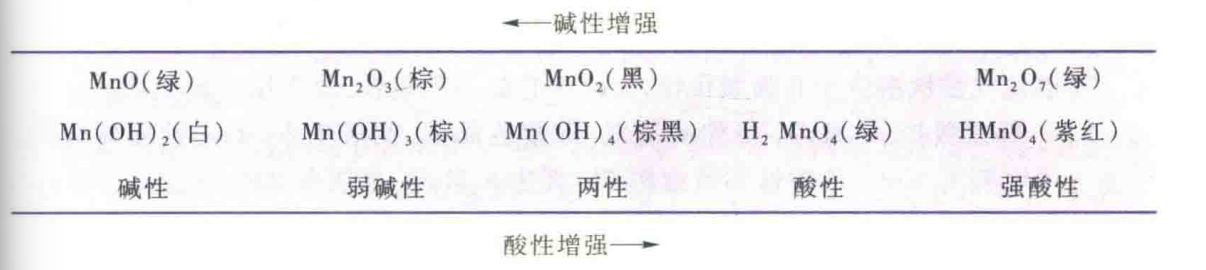
\includegraphics[width=0.8\textwidth]{figure//锰的变化.png}
	\caption{锰的氧化物、水合物酸碱性递变规律}
	\label{fig:}
\end{figure}

1.锰(II)盐

溶解性:锰(II)的强酸盐均溶于水,少数弱酸(碳酸、氢硫酸)盐难溶。

颜色:由于结晶都带有淡红\ce{[Mn(H2O)6]^2+},因此溶液呈现淡红色。

与碱反应:产生白色胶状\ce{Mn(OH)2}迅速被空气氧化为棕色\ce{MnO(OH)2}(水合二氧化锰):

$$ \ce{Mn^2+ + 2OH- -> Mn(OH)2(\text{白色})} $$

$$ \ce{2Mn(OH)2 + O2 -> 2MnO(OH)2(\text{棕色})} $$

鉴定:用强氧化剂(铋酸钠,二氧化铅,过硫酸铵)可将稳定的\ce{Mn^2+}氧化为紫红色高锰酸根,如:

$$ \ce{2Mn^2+ + 14H+ + 5NaBiO3 -> 2MnO4- + 5Bi^3+ + 7H2O + 5Na+} $$

2.二氧化锰

物理性质:\ce{MnO2}为棕色黑色粉末,极其稳定。

氧化性:在酸性溶液有强氧化性,可氧化出氯气:

$$ \ce{MnO2 + HCl(\text{浓}) -> MnCl2 + Cl2 + 2H2O} $$

还原性:与碱共熔生成绿色锰酸盐:

$$ \ce{2MnO2 + 4KOH + O2 ->[\text{熔融}] 2K2MnO4(\text{绿色}) + 2H2O} $$

3.锰酸盐、高锰酸盐

(1)锰酸盐。氧化数为+6的锰的化合物,仅存在于强碱中,深绿色。

制备:在空气或其他氧化剂存在时,令\ce{MnO2}与碱金属氢氧化物或碳酸盐共熔制得,如:

$$ \ce{3MnO2 + 6KOH + KClO3 ->[\text{熔融}] 3K2MnO4 + KCl + 3H2O} $$

歧化:之前提到,在酸性溶液中发生歧化;在碱中也发生,但速率很低。

(2)高锰酸盐。俗称灰锰氧,深紫色晶体,能溶于水,强氧化剂。

制备:电解锰酸钾碱性溶液或用\ce{Cl2}氧化锰酸钾:

$$ \ce{2MnO4^2- + Cl2 -> 2MnO4- + 2Cl-} $$

稳定性:受光催化在酸中分解:

$$ \ce{4MnO4- + 4H+ -> 4MnO2 v + 3O2 ^ + 2H2O} $$

保存在棕色瓶中。

氧化性:在酸性、中性、强碱性介质中还原产物分别为\ce{Mn^2+(\text{淡红色}),MnO2(\text{棕色}),MnO4^2-(\text{绿色})}。

颜色:尽管为\ce{MnO4-}为$3d^0$,但由于\ce{Mn-O}之间存在较强极化效应,产生荷移跃迁,令其呈紫色,同样的情况还包括\ce{VO4^3-(\text{黄色}),CrO4^2-(\text{黄色}),MoO4^2-(\text{淡黄色}),MnO4^2-(\text{绿色})}。

荷移跃迁:原子或离子团吸收可见光后使电子从负电荷粒子向正电荷粒子跃迁。

\subsection{铁系和铂系元素}

\subsubsection{概述}

铁系:第一过渡系的铁、钴、镍。

铂系:d区第VIII族元素除了铁钴镍剩余的6种元素:\ce{Ru,Rh,Pd,Os,Ir,Pt}。

铂系元素与金银一起称为贵金属元素。

1.铁系元素

由于VII族d层电子已超过5个(半满),全部d电子不再能参与成键,所以铁系不像前面的过渡元素易形成\ce{VO3-,CrO4^2-,MnO4-}那样的含氧酸根离根离子。

铁的氧化数为+2,+3,其中+3的化合物最稳定;钴的氧化数为+2,+3,其中+2的化合物最稳定。镍主要形成+2的化合物。

铁磁性物质:具有磁性,在外加磁场作用下,磁性增强,外磁场移走后仍保持磁性的物质称为铁磁性物质。铁钴镍都是铁磁性物质。

活泼性:活泼性都大于氢,都可被浓硝酸钝化;铁能被浓碱侵蚀,但钴和镍不会(镍坩埚)。

氢脆:钢铁与氢作用生成氢化物会使钢铁的延展性和韧性下降。

合金钢:在钢中加入一定量其他元素,如不锈钢、铸铁等。\\

2.铂系元素

自然界中铂系元素在矿物中以单质状态存在。

铂系元素形成高氧化态的倾向从左向右逐渐减小,从上到下逐渐增加。

大多数铂系元素能吸收气体,钯的吸氢能力最大。

铂系元素化学稳定性很高,常温下与大多数非金属元素(包括氧、氯)都不反应,钯和铂能溶于王水:

$$ \ce{3Pt + 4HNO3 + 18HCl -> 3H2[PtCl6] + 4NO ^ + 8H2O} $$

\ce{Ru,Rh,Os,Ir}甚至不溶于王水。

\subsubsection{铁钴镍的化合物}

1.氧化物和氢氧化物

(1)氧化物。铁钴镍均可形成+2,+3氧化数的有色氧化物:

\begin{tabular}{c|c|c}
\ce{FeO} &\ce{CoO}  &\ce{NiO}\\ \hline
黑色&灰绿色&暗绿色\\
\ce{Fe2O3}&\ce{Co2O3}&\ce{Ni2O3}\\ \hline
砖红色&黑色&黑色\\
\end{tabular}

铁还能形成混合价态氧化物\ce{Fe3O4}。

酸碱性:铁钴镍的+2,+3氧化数的氧化物均能溶于强酸,不溶于水和碱,是碱性氧化物。

氧化性:\ce{M2O3}的氧化能力按照\ce{Fe-Co-Ni}的顺序递增,稳定性递降,如与盐酸反应\ce{Fe2O3}只生成三价盐,但\ce{Ni2O3}生成二价盐和氯气。\\

\begin{tcolorbox}
	
	为什么\ce{M2O3}型氧化物稳定性按照铁-钴-镍顺序递降,而氧化性递增?\\

	一般氧化性越强,稳定性越低,因为越容易被还原。

	而铁系元素氧化性与其3d轨道单电子数目有关,单电子数目越多,氧化性越弱。

	铁、钴、镍轨道中单电子分别有4、3、2个,因此M2O3氧化性按照铁-钴-镍顺序递增。

\end{tcolorbox}


(2)氢氧化物。

溶解性:铁系元素的氢氧化物均难溶于水,氧化还原性及其变化规律与其氧化物类似:

\begin{figure}[htpb]
	\centering
	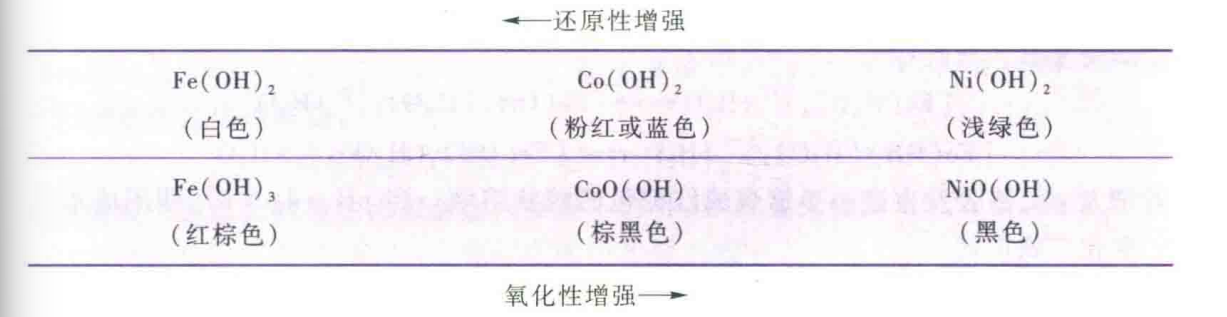
\includegraphics[width=0.8\textwidth]{figure//铁系氢氧化物.png}
	\caption{铁系氢氧化物的氧化还原性及变化规律}
	\label{fig:}
\end{figure}

稳定性:\ce{Fe(OH)2}很不稳定,在生成后随即被空气氧化为红棕色\ce{Fe(OH)3}。

\ce{Co(OH)2}较\ce{Fe(OH)2}稳定,但在空气中被缓慢氧化为棕黑色\ce{CoO(OH)}。

\ce{Ni(OH)2}更稳定,除非与强氧化剂作用才变为黑色\ce{NiO(OH)}。

氧化性:氧化性与稳定性相反,按照铁-钴-镍顺序递增。例如,\ce{Fe(OH)3}只能中和盐酸,但\ce{CoO(OH)}能氧化盐酸,生成氯气。

$$ \ce{2CoO(OH) + 6HCl -> 2CoCl2 + Cl2 ^ + 4H2O} $$

2.盐类

(1)M(II)盐。氧化数为+2的铁钴镍盐,性质相似:

溶解性:强酸盐都易溶于水,有微弱水解,显酸性。强酸盐析出带有一定结晶水,呈现各种颜色。硫酸盐都能和碱金属或铵的硫酸盐形成复盐,如硫酸亚铁铵\ce{(NH4)2SO4 * FeSO4 * 6H2O}(莫尔盐)比亚铁盐更稳定,不易氧化。

\ce{CoCl2 * 6H2O}在受热脱水时伴有颜色变化,从粉红变为蓝色,用作硅胶变色剂。

(2)M(III)盐。铁系中只有铁能形成稳定的+3简单盐。

酸碱性:\ce{Fe(OH)3}的碱性比\ce{Fe(OH)2}弱,所以三价铁盐比二价铁盐更容易水解。

氧化性:中强氧化剂,可氧化铜单质、碘离子等。\\

3.配合物

(1)氨合物。\ce{Fe^2+,Co^2+,Ni^2+}都能形成氨合配离子,稳定性依照\ce{Fe^2+,Co^2+,Ni^2+}顺序依次增强,正好与三价氧化物稳定性相反(原因是向右中心离子半径减小、对配体吸引力增强,稳定性增强)。

但是,\ce{Fe^2+}的氨合物(\ce{[Fe(NH3)6]Cl2})遇水分解;\ce{Fe^3+}强烈水解,加入氨无法形成氨合物,而是生成\ce{Fe(OH)3}沉淀。

\ce{Co^2+}与过量氨水反应生成土黄色\ce{[Co(NH3)6]^2+},在空气中被慢慢氧化为红褐色\ce{[Co(NH3)6]^3+}:

$$ \ce{4[Co(NH3)6]^2+ + O2 + 2H2O -> 4[Co(NH3)6]^3+ + 4OH-} $$

虽然\ce{Co^3+}很不稳定,氧化性很强,但\ce{Co(III)}氨合物氧化性减弱,稳定性大幅增强。

\ce{Ni^2+}在过量氨水中生成较稳定蓝色\ce{[Ni(NH3)6]^2+}。\\

(2)氰合物。

\ce{Fe(II)}盐与\ce{KCN}溶液作用得到白色\ce{Fe(CN)2}沉淀,过量时溶解生成\ce{[Fe(CN)6]^4-}:

$$ \ce{Fe^2+ + 2CN- -> Fe(CN)2 v (\text{白色})} $$

$$ \ce{Fe(CN)2 + 4CN- -> [Fe(CN)6]^4-} $$

黄血盐:上述溶液析出的黄色晶体\ce{K4[Fe(CN)6] * 3H2O}。黄血盐可以被氧化剂氧化为深红色赤血盐\ce{K3[Fe(CN)6]}。

鉴定:黄血盐和赤血盐均用来检验与自己价态不同的(+2,+3中)的(亚)铁离子,生成同一种蓝色沉淀\ce{[KFe(CN)6Fe]}。

\ce{Co^2+}与\ce{CN-}反应,先形成浅棕色沉淀,之后形成茶绿色溶液,易被空气中氧化为黄色六氰合钴。

\ce{Ni^2+}与\ce{CN-}反应,先生成灰蓝色沉淀,之后形成橙黄色溶液。\\

(3)硫氰合物。\ce{Fe^3+}与\ce{SCN-}反应生成血红色\ce{[Fe(NCS)_n]^{3-n}},可用于鉴定铁离子。

\ce{Co^2+}与\ce{SCN-}反应,生成蓝色\ce{[Co(NCS)4]^2-},此反应用于鉴定\ce{Co^2+},用水稀释变为粉红色\ce{Co(H2O)6]^2+}。

\ce{Ni^2+}与\ce{SCN-}反应生成配合物不太稳定。\\

(4)羰合物、螯合物。

见P356。

\section{过渡元素(二)}

\subsection{铜族元素}

\subsubsection{铜族元素通性}

铜族元素位于元素周期表ds区IB族,包含铜(\ce{Cu})、银(\ce{Ag})、金(\ce{Au})、錀(\ce{Rg})。

铜、银主要以硫化物、氧化物矿的形式存在;铜、银、金均有单质状态存在的矿物。

铜族元素原子价层电子构型为$(n-1)d^{10}ns^{1}$,氧化数有+1,+2,+3;

铜、银、金最常见的氧化数分别为+2、+1、+3 。(铜、金非+1的原因可参考它们的氧化电极电势,并且\ce{Cu^{+}}在水中容易与水结合,导致能量变化,易歧化为0、+2价)

$$ E^{\Theta}_{A}/V \quad \ce{Cu^{3+} \overset{2.4}{\text{------}} Cu^{2+} \overset{0.159}{\underset{}{\text{------}}} Cu+ \overset{0.520}{\underset{}{\text{------}}} Cu}$$

$$ E^{\Theta}_{A}/V  \quad \ce{Ag^{3+} \overset{1.8}{\underset{}{\text{------}}} Ag^{2+} \overset{1.980}{\underset{}{\text{------}}} Ag+ \overset{0.7991}{\underset{}{\text{------}}} Ag} $$




铜族金属离子有较强的极化力,本身变形性大,二元化合物有相当的共价型(如\ce{CuCl2}为共价化合物)。

与其他过渡金属类似,易形成配合物。\\$\Delta$原因:(1)过渡元素有能量相近的未充满的(n-1)d,ns,np价轨道,属于同一能级组,可以通过不同杂化方式形成杂化轨道,接受配体提供的孤对电子,有的还可以形成d-p反馈$\pi$键。(2)过渡金属电子层数增加慢,钻穿效应强,有效核电荷数多,有利于作为中心原子吸引配体。

\subsubsection{铜族元素单质}
熔沸点相对较低,硬度小,有极好延展性和可塑性;导热、导电能力极强,\ce{Cu}是最通用导体。

银、金熔体能从空气中吸收大量氧气,冷凝时又释放。

银、铜、金能与多种金属形成合金。

银、铜、金的化学活泼性差;\ce{Cu}在潮湿空气中生成铜绿:

$$ \ce{2Cu + O2 + CO2 -> Cu2(OH)2CO3} $$

银的化学活泼性在铜、金之间,在室温下不与氧气、水反应,在高温不与氢、氮、碳反应,与卤素反应较慢。在室温下与含有\ce{H2S}的空气反应会生成深色\ce{Ag2S}。

$$ \ce{4Ag + 2H2S + O2 -> 2Ag2S + 2H2O} $$

铜,银仅与氧化性酸反应:与稀硝酸生成硝酸盐和\ce{NO},与浓硝酸生成硝酸盐和\ce{NO2},与热的浓硫酸反应生成\ce{SO2}

高温下与氧气不反应的只有金。

金不溶于单一无机酸,但溶于王水:

$$ \ce{Au + HNO3 + 4HCl ->H[AuCl4] + NO ^ + 2H2O} $$

银遇王水产生\ce{AgCl}薄膜阻止反应继续进行。

\subsubsection{铜的重要化合物}
1.氧化物和氢氧化物\\

\ce{CuO}:

加热分解硝酸铜和碳酸铜可得黑色\ce{CuO};\ce{Cu(OH)2}受热分解脱水也生成\ce{CuO}

\ce{CuO}加热可分解为暗红色\ce{Cu2O}

$$ \ce{4CuO ->[1000^\circ C] 2Cu2O + O2} $$

\ce{CuO}是高温超导材料。\\

\ce{Cu(OH)2}:

\ce{Cu(OH)2}显两性(以弱碱性为主),既溶于酸也溶于浓强碱,在强碱中生成四羟基合铜离子。

\ce{[Cu(OH)4]2-}可被葡萄糖还原为暗红色的\ce{Cu2O}

$$ \ce{[2Cu(OH)4]2- C6H12O6 -> Cu2O v + C6H12O7 + 4OH- + 2H2O} $$

\ce{Cu(OH)2}易溶于氨水,生成深蓝色\ce{[Cu(NH3)4]^{2+}}。\\

\ce{CuCl}和\ce{Cu2O}:

\ce{CuCl}难溶于水,溶于氨水和浓盐酸并生成配合物。

向\ce{CuCl}的盐酸冷溶液中加入\ce{NaOH},生成黄色\ce{CuOH}沉淀,但沉淀很快变为橙色,最后变为红色\ce{Cu2O}。

\ce{Cu2O}热稳定性很强,难溶于水,但是易溶于稀酸,并立即歧化为\ce{Cu^{2+}}和\ce{Cu}。

$$ \ce{Cu2O + 2H+ -> Cu^{2+} + Cu + H2O} $$

与盐酸则反应生成难溶于水的\ce{CuCl}

$$ \ce{Cu2O + 2HCl -> CuCl + H2O} $$

溶于氨水,形成无色配离子\ce{[Cu(NH3)2]^{+}}

$$ \ce{Cu2O + 4NH3 + H2O -> [Cu(NH3)2]^{+} + 2OH-} $$

但\ce{[Cu(NH3)2]^{+}}遇到空气就被氧化为深蓝色\ce{[Cu(NH3)4]^{2+}}

$$ \ce{4[Cu(NH3)2]^{+} + O2 + 8NH3 + 2H2O -> 4[Cu(NH3)4]^{2+} + 4OH-} $$\\

\ce{[Cu(NH3)2]OAc}可以吸收\ce{CO}。

$$ \ce{[Cu(NH3)2]OAc + CO + NH3 <=>[\text{低温加压}][\text{升温减压}] [Cu(CO)(NH3)3]OAc} $$

\ce{Cu2O}可用作红色颜料。\\

2.盐类

(1)氯化亚铜

向热的浓盐酸中用铜还原\ce{CuCl2}可以生成无色\ce{[CuCl2]-}配合物,用水稀释即可生成白色\ce{CuCl}沉淀。

$$ \ce{Cu + Cu^{2+} + 4Cl- -> 2[CuCl2]-} $$

$$ \ce{2[CuCl2]- -> 2CuCl + 2Cl-} $$

用还原剂\ce{SnCl2}也可以得到\ce{CuCl}。

$$ \ce{2CuCl2 + SnCl2 -> 2CuCl v + SnCl4} $$

另外,\ce{CuCl}还可以吸收\ce{CO}生成氯化羰基亚铜(\ce{[Cu(CO)Cl] * H2O})

$$ \ce{CuCl + CO + H2O -> [Cu(CO)Cl] * H2O} $$

该反应可用于测定有机反应中\ce{CO}的产生量。

(2)氯化铜

\ce{CuCl2}是一种棕黄色固体,可由单质直接化合而成,是一种共价化合物,结构为\ce{CuCl4}组成的长链。

\begin{figure}[htpb]
	\centering
	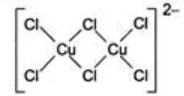
\includegraphics[width=0.3\textwidth]{figure//Cu结构.png}
	\caption{Cu结构}
	\label{fig:Cu结构}
\end{figure}

\ce{CuCl2}不仅易溶于水,而且易溶于有机溶剂,如乙醇,丙酮等。在很高浓度\ce{CuCl2}溶液中,可形成黄色配合物\ce{[CuCl4]^{2-}},显黄色。

$$ \ce{Cu^{2+} + 4Cl- -> [CuCl4]^{2-}} $$

在\ce{CuCl2}稀溶液中,由于被\ce{[Cu(H2O)4]^{2+}}取代,显浅蓝色。

$$ \ce{[CuCl4]^{2-} + 4H2O -> [Cu(H2O)4]^{2+} + 4Cl-} $$

所以,\ce{CuCl2}高浓度溶液常显黄色或黄绿色,这是两种配离子都存在的缘故。

(3)硫酸铜

无水硫酸铜为白色粉末,在水中结晶时为五水合硫酸铜,呈蓝色。五水合硫酸铜(\ce{[Cu(H2O)5]SO4})俗称胆巩,其结构为\ce{[Cu(H2O)4]SO4 * H2O},4个水分子与\ce{Cu^{2+}}配位,1个水分子通过氢键与\ce{SO4^{2-}}结合。温度升高,水逐渐脱去。

无水硫酸铜易溶于水,吸水性强,吸水则显出特征性蓝色,可用于测量气体微量水分和作为干燥剂。\ce{CuSO4}由于铜离子水解而呈弱酸性。

\ce{CuSO4}具有杀菌性,可制备波尔多液。\\

3.配合物

(1)\ce{Cu}(I)的配合物:

\ce{Cu}(I)通常形成配位数为2的配合物,常见的有:

\ce{[Cu(SCN)2]+},\ce{[CuCl2]-},\ce{[Cu(NH3)2]+},\ce{[Cu(S2O3)]^{2-}},\ce{[Cu(CN)2]-}

由于\ce{Cu+}的价电子结构为$d^{10}$型,形成的配离子基本无色,大多配合物溶液有吸收\ce{CO}、烯烃、炔烃和释放的能力。

$$ \ce{[Cu(NH2CH2CH2OH)2]+ + C2H4 <=> [Cu(NH2CH2CH2OH)2(C2H4)]+} \Delta _{f}H^{\Theta}_{m}<0$$

该反应常用于石油中分离烯烃。

(2)\ce{Cu}(II)的配合物:

\ce{Cu}(II)与单齿配体通常形成配位数为4的正方形配合物,例如\ce{[CuCl4]2-},\ce{[Cu(NH3)4]^{2+}},\ce{[Cu(H2O)4]^{2+}}。

过量氨水与\ce{Cu^{2+}}盐溶液反应可以生成\ce{[Cu(NH3)4]^{2+}}。

$$ \ce{[Cu(H2O)4]^{2+} + 4NH3 -> [Cu(NH3)4]^{2+} + 4H2O} $$

溶液中\ce{Cu^{2+}}的浓度越小,所形成的蓝色\ce{[Cu(NH3)4)]^{2+}}的颜色越浅,可根据此判断溶液中\ce{Cu^{2+}}含量;\ce{[Cu(NH3)4]^{2+}}有溶解纤维的能力,加入酸或水后纤维又可以析出,工业上利用这种性质制造人造丝。

4.铜(I)与铜(II)的相互转化

虽然\ce{Cu+}为$3d^{10}$结构,但在水溶液中易歧化。由于\ce{Cu^{2+}}所带电荷比\ce{Cu+}多,并且水合焓代数值远远小于\ce{Cu+},所以在水溶液中\ce{Cu+}不如\ce{Cu^{2+}}稳定。

酸性溶液中,\ce{Cu+}的水解常数很大,反应进行得很彻底。而要使\ce{Cu+}转化为\ce{Cu^{2+}},则需要还原剂或者减低\ce{Cu+}的浓度,让它成为难溶物或者难解离的配合物,例如氯化亚铜的制备。

$E_{A}^{\Theta}/V(\ce{Cu^{2+}/CuCl}) 大于 E_{A}^{\Theta}/V(\ce{CuCl/Cu})$,所以\ce{Cu^{2+}}可将\ce{Cu}氧化为\ce{CuCl}。用\ce{SO2}代替\ce{Cu}:

$$ \ce{2Cu^{2+} + SO2 + 2Cl- + 2H2O -> 2CuCl v + SO4^{2-} + 4H+} $$

或者\ce{Cu^{2+}}与\ce{KI}反应,可以得到白色的\ce{CuI}沉淀。

$$ \ce{2Cu^{2+} + 4I- -> 2CuI v + I2} $$

由于$E^{\Theta}_{A}(\ce{Cu^{2+}/CuI})大于E^{\Theta}_{A}(\ce{I2/I-})$,所以\ce{Cu^{2+}}与\ce{I-}反应得不到沉淀\ce{CuI2},而是得到沉淀\ce{CuI}。

\begin{tcolorbox}
原理:

根据反应电动势与反应常数的关系可知:

$ lgK^{\Theta} = \frac{z * E_{MF}}{0.0592V} $

氧化还原电对电动势越高,反应常数越大,越容易反应完全。所以,生成\ce{CuI}的反应反应常数大于\ce{CuI2}的,生成\ce{CuI}。
\end{tcolorbox}

同样地,向热的\ce{Cu(II)}盐溶液中加入\ce{KCN},可以得到白色的\ce{CuCN}沉淀。

$$ \ce{2Cu^{2+} + 4CN- -> 2CuCN v + (CN)2 ^} $$

继续加入过量的KCN,\ce{CuCN}形成\ce{Cu(I)}最稳定的配离子\ce{[Cu(CN)x]^{1-x}}而溶解。

$$ \ce{CuCN + (x-1)CN- -> [Cu(CN)_{x}]^{1-x}} (x=2\sim 4)$$

$\Delta$ 总之,在水溶液中,凡能使\ce{Cu+}生成难溶盐或者稳定\ce{Cu(I)}配离子时,则可使\ce{Cu(II)}转化为\ce{Cu(I)}化合物。


\subsubsection{银的重要化合物}

1.氧化物与氢氧化物

\ce{AgOH}只有用强碱与可溶性银盐的90\%酒精溶液在低于零下40$^\circ C$才能制得。AgOH为白色固体,极不稳定,形成后立即脱水为暗棕色\ce{Ag2O}

$$ \ce{2Ag+ + 2OH- -> Ag2O + H2O} $$

与\ce{Cu2O}相比,\ce{Ag2O}的碱性略强,但是热稳定性差,稍加热便分解为单质和氧。

\ce{Ag2O}既能与硝酸反应,也能溶于氨水,形成二氨合银。

$$ \ce{Ag2O + 4NH3 + H2O -> 2[Ag(NH3)2]+ + 2OH-} $$

2.卤化银

卤化银中只有\ce{AgF}溶于水。卤化银颜色随着\ce{Cl-Br-I}顺序加深,溶解度依次降低。卤化银有感光性,在光照下被分解为单质,先变为紫色,后变为黑色。

$$ \ce{2AgX ->[\text{日光}] 2Ag + X2} $$

\begin{tcolorbox}
原理:

生成的银单质结构松散,没有形成金属晶体,不存在导带,故没有金属光泽,显黑色。

溶解度则是因为阴离子变形性不断增大,极化作用不断增强,共价成分增大,在水中逐渐难溶。

\end{tcolorbox}

\ce{AgBr}可被硫代硫酸钠溶解,形成可溶配合物:

$$ \ce{AgBr + 2S2O3^{2-} -> [Ag(S2O3)2]^{3-} + Br-} $$

该反应曾被用作得到底片。

3.硝酸银

制备:使用蒸发结晶法。

\ce{AgNO3}受热或遇光照容易分解为\ce{NO2}和\ce{O2}。

$$ \ce{2AgNO3 ->[\text{713K或光照}] 2Ag + 2NO2 ^ + O2 ^} $$

\ce{AgNO3}具有氧化性,遇微量有机物即被还原为黑色的单质银。

4.配合物

常见与\ce{Ag+}形成二配合物的有:\ce{NH3},\ce{SCN-},\ce{S2O3^{2-}},\ce{CN-},他们形成的配离子稳定性逐渐增加。

\begin{tcolorbox}

原理:

一般来说,单齿配合物稳定性比多齿配合物要强;配体电负性越大,配合键共价性越强,越具有稳定性;配体的分子量越大,与中心原子距离越远,配合键越不稳定。\\

\ce{CN-}是单齿配体,电负性很强,所以稳定性最强;\ce{S2O3^{2-}}虽然为双齿配体,但是电负性较强,其次;\ce{SCN-}虽是单齿配体,但是配位原子可能是\ce{S}也可能是\ce{N},不稳定;\ce{NH3}为单齿,但\ce{N}原子电负性最低,且空间占据大,配合键键长较大,不稳定。

\end{tcolorbox}

二氨合银离子具有弱氧化性,银镜反应:

$$ \ce{2[Ag(NH3)2]+ + RCHO + 3OH- -> 2Ag v + RCOO- + 4NH3 ^ + 2H2O} $$

\ce{2[Ag(NH3)2]+}放置过程中会变成有爆炸性的\ce{Ag2NH}和\ce{AgN3}。

\subsection{锌族元素}

\subsubsection{锌族元素概述}

1.锌族元素通性

周期表$ds$区包括锌(\ce{Zn})、镉(\ce{Cd})、汞(\ce{Hg})及鎶(\ce{Cn})。\\

对于闪锌矿(\ce{ZnS}),通常使用先焙烧为\ce{ZnO},再用焦炭还原提纯\ce{Zn}。

或者使用湿法,使用硫酸和氧气把\ce{ZnS}转化为\ce{ZnSO4}和硫单质,之后对\ce{ZnSO4}使用电解。\\

锌族元素的价层电子构型均为$(n-1)d^{10}ns^{2}$,由于(n-1)d层电子未成键,所以锌族元素性质与典型过渡元素有较大差别,与p区元素较接近。氧化数主要为+2,汞有+1(总是以双聚离子\ce{[--Hg--Hg--]^{2-}}形式存在),离子无色,金属键较弱,所以硬度低,熔点低。\\

就活泼性而言,除\ce{Hg}之外,\ce{Zn}、\ce{Cd}是较活泼金属;\ce{Zn}和\ce{Cd}的化学性质比较接近,\ce{Hg}与它们相差较大,更接近于铜族元素。\\

锌族元素的\ce{M^{2+}}均无色,所以它们的许多化合物也无色。但是,由于\ce{M^{2+}}具有18电子构型,其极化能力和变形性依\ce{Zn^{2+}--Cd^{2+}--Hg^{2+}}的顺序增强,导致\ce{Cd^{2+}}特别是\ce{Hg^{2+}}与易变形的阴离子形成的化合物,往往显色并具有较低的溶解度。(注:由于锌族元素的阳离子较大较特殊,在判断离子极化时主要考虑其变形性)\\

锌族元素一般都形成较稳定的配合物。

2.锌族单质

锌、镉、汞均为银白色金属,其中锌略带蓝白色。本族元素单质熔沸点较低,并按照从上到下的顺序降低。(原因:同族元素从上到下原子半径增大,金属键减弱)

锌可与其他金属形成许多合金。

汞能溶解许多金属形成汞齐,汞齐是汞的合金。钠汞齐与水反应放出氢,在有机合成中常常用作还原剂。利用汞与金属形成汞齐的特点可从矿石中提取金银等。

锌和镉的化学性质相似,而汞的化学活泼性差很多:

$$ \ce{2Zn + O2 ->[1000^\circ C] 2ZnO} $$
$$ \ce{2Hg + O2 <=>[\text{加热至沸}][500^\circ C] 2HgO} $$

锌在潮湿空气中表面生成一层的致密碱式碳酸盐\ce{Zn(OH)2 * ZnCO3}起保护作用,使锌具有防腐蚀的性能。

$$ \ce{2Zn + O2 + H2O + CO2 -> Zn(OH)2 * ZnCO3} $$

锌与铝相似,具有两性:

$$ \ce{Zn + 2H+ -> Zn^{2+} + H2 ^} $$
$$ \ce{Zn + 2OH- + 2H2O -> [Zn(OH)4]^{2-} + H2 ^} $$

与铝不同的是,\ce{Zn}能与氨水形成配离子而溶解:

$$ \ce{Zn + 4NH3 + 2H2O -> [Zn(NH3)4](OH)2 + H2 ^} $$

\subsubsection{锌的重要化合物}

1.氧化锌和氢氧化锌

氧化锌(\ce{ZnO})又称锌白,对热稳定,微溶于水,显两性。

在锌盐溶液中,加入适量的碱可析出\ce{Zn(OH)2}沉淀。\ce{Zn(OH)2}也显两性,溶于碱生成锌酸盐:

$$ \ce{Zn(OH)2 + 2OH- -> [Zn(OH)4]^{2-}} $$

也可以溶于氨水,形成配合物:

$$ \ce{Zn(OH)2 + 4NH3 -> [Zn(NH3)4]^{2+} + 2OH-} $$

\begin{tcolorbox}

为什么\ce{Zn}和\ce{Al}拥有两性?\\

与一般的硫酸盐、硝酸盐的组成有很大的不同。对于一般的金属,它们一般表现出金属性,即与由非金属元素与氧组成的酸根阴离子结合;然而像\ce{Zn}、\ce{Al}这样的金属,它们随着原子半径的增大和原子层数的增加,也能表现出一些非金属性,与\ce{O}结合成为阴离子,即常说的两性。

所以,锌酸根可以写作\ce{[Zn(OH)4]^{2-}},也可以写作\ce{ZnO2^{2-}}。

\end{tcolorbox}

2.氯化锌

无水氯化锌为白色固体,可由锌与氯气反应制得。

\ce{ZnCl2}吸水性很强,极易溶于水,水溶液由于锌离子的水解显酸性。

$$ \ce{Zn^{2+} + H2O <=> Zn(OH)+ + H+} $$

在\ce{ZnCl2}的浓溶液中,由于形成配合酸\ce{H[ZnCl2(OH)]},而让溶液具有显著的酸性,甚至能溶解金属氧化物:

$$ \ce{ZnCl2 + H2O -> H[ZnCl2(OH)]} $$

$$ \ce{Fe2O3 + 6H[ZnCl2(OH)] -> Fe[ZnCl2(OH)]3 + 3H2O} $$

在焊接金属前,常用\ce{ZnCl2}的浓溶液清除金属表面的氧化物。\\

要得到无水氯化锌,可用含水氯化锌与氯化亚砜(\ce{SOCl2})一起加热:

$$ \ce{ZnCl2 * xH2O + xSOCl2 -> ZnCl2 + 2xHCl + xSO2} $$

3.硫化锌

往锌盐溶液中通入\ce{H2S}时,会生成\ce{ZnS}。

\ce{ZnS}是常见难溶硫化物中唯一呈白色的,与\ce{BaSO4}共同沉淀所形成的混合物晶体\ce{ZnS * BaSO4}叫做锌钡白(俗称立德粉)。\\

在\ce{ZnS}中加入微量\ce{Cu}、\ce{Mg}、\ce{Ag}作活化剂,经光照射后可发出不同颜色的荧光。

4.配合物

\ce{Zn^{2+}}与氨水、氰化钾等可形成无色的四配位的配离子。\\

\ce{[Zn(CN)4]^{2-}}用于电镀工艺。值得注意的是,铜、锌配合物有关电对的标准电极电势相近,所以它们的混合液在电镀时,\ce{Zn}、\ce{Cu}在阴极同时析出,即镀黄铜。

$\Delta$\ce{Zn^{2+}}与二苯硫腙形成稳定的粉色螯合物沉淀,用于鉴定。

\subsubsection{汞的重要化合物}

汞能形成氧化物为+1,+2的化合物,在锌族M(I)的化合物中,以\ce{Hg(I)}的化合物最重要。\\

1.氧化汞

氧化汞有两种红、黄两种变体,都难溶于水,有毒,在500$^\circ C$时分解为汞和氧气。在汞盐溶液中加入碱,可得到黄色\ce{HgO},原因与\ce{Ag}类似,生成的\ce{Hg(OH)2}极不稳定,立即脱水分解。红色的\ce{HgO}则一般由硝酸汞受热分解制得。

$$ \ce{Hg^{2+} + 2OH- -> HgO v + H2O} $$

$$ \ce{2Hg(NO3)2 ->[\Delta] 2HgO + 4NO2 + O2 ^} $$

\ce{HgO}是制备许多汞盐的原料。\\

2.氯化汞和氯化亚汞

氯化汞可由在过量氯气中加热汞制得。

\ce{HgCl2}为共价化合物,熔点较低,易生化,俗称升汞。略溶于水,在水中解离度很小,主要以分子形式存在,有“假盐”之称。

\ce{HgCl2}在水中稍微水解:

$$ \ce{HgCl2 + H2O <=> Hg(OH)Cl + HCl} $$

与稀氨水反应则生成难溶的氨基氯化汞:

$$ \ce{HgCl2 + 2NH3 -> Hg(NH2)Cl v (\text{白色}) + NH4Cl} $$

\ce{HgCl2}还可以与碱金属氯化物反应形成四氯合汞(II)配离子,让\ce{HgCl2}的溶解度增大。

$$ \ce{HgCl2 + 2Cl- -> [HgCl4]^{2-}} $$

\ce{HgCl2}在酸性溶液中有氧化性,适量的\ce{SnCl2}可以将之还原为难溶于水的白色氯化亚汞。

$$ \ce{2HgCl2 + SnCl2 -> Hg2Cl2 v (\text{白色}) + SnCl4} $$

分析化学中用此反应鉴定Hg(II)和Sn(II)。\ce{HgCl2}的稀溶液有杀菌作用。\\

金属汞与\ce{HgCl2}固体一起研磨,制得氯化亚汞。

$$ \ce{2Hg + 2HgCl2 -> 2Hg2Cl2} $$

氯化亚汞(\ce{Hg2Cl2}为白色固体,难溶于水。少量的\ce{Hg2Cl2}无毒,俗称甘汞,见光易分解。

$$ \ce{Hg2Cl2 ->[\text{光}] HgCl2 + Hg} $$

\ce{Hg2Cl2}与氨水反应可生成氨基氯化汞和汞,令沉淀显灰色:

$$ \ce{Hg2Cl2 + 2NH3 -> Hg(NH3)Cl v (\text{白色}) + Hg(\text{黑色}) + NH4Cl} $$

此反应可用于鉴定\ce{Hg(I)}。\\

3.硝酸汞和硝酸亚汞

硝酸汞\ce{[Hg(NO3)2]}和硝酸亚汞\ce{[Hg2(NO3)2]}都溶于水,并且水解生成碱式盐沉淀。

$$ \ce{Hg(NO3)2 + H2O -> HgO * Hg(NO3)2 v + 2HNO3} $$

$$ \ce{Hg2(NO3)2 + H2O -> Hg2(OH)NO3 v + HNO3} $$

所以在配置它们的溶液时,应先溶于稀硝酸中。

在\ce{Hg(NO3)2}中加入\ce{KI}可产生橘红色\ce{HgI2}沉淀,后者溶于过量\ce{KI}中,形成无色\ce{[HgI4]^{2-}}:

$$ \ce{Hg^{2+} + 2I- -> HgI2 v (\text{橘红色})} $$

$$ \ce{HgI2 + 2I- -> \ce{[HgI4]^{2-}}} $$

同样地,在\ce{Hg2(NO3)2}溶液中加入\ce{KI},先生成浅绿色的\ce{Hg2I2}沉淀,再加入\ce{KI}后形成\ce{[HgI4]^{2-}},同时有汞析出:

$$ \ce{Hg2^{2+} + 2I- -> Hg2I2 v (\text{浅绿色})} $$

$$ \ce{Hg2I2 +  2I- -> [HgI4]^{2-} + Hg v} $$

在\ce{Hg(NO3)2}溶液中加入氨水,可得白色的氨基硝酸汞沉淀。

$$ \ce{2Hg(NO3)2 + 4NH3 + H2O -> HgO * NH2HgNO3 v (\text{白色}) + 3NH4NO3} $$

在硝酸亚汞中加入氨水会产生上述沉淀和单质汞。

$$ \ce{2Hg2(NO3)2 + 4NH3 + H2O -> HgO * NH2HgNO3 v (\text{白色}) + 3NH4NO3 + 2Hg(\text{黑色})} $$

\ce{Hg2(NO3)2}受热易分解:

$$ \ce{Hg2(NO3)2 ->[\Delta] 2HgO + 2NO2 ^} $$

由于氧-水电势高于汞离子-亚汞离子的,所以当\ce{Hg2(NO3)2}溶液与空气接触时易被氧化为\ce{Hg(NO3)2}:

$$ \ce{2Hg2(NO3)2 + O2 + 4HNO3 -> 4Hg(NO3)2 + 2H2O} $$

因此可加入少数金属汞避免\ce{Hg2(NO3)2}溶液被氧化。

汞能形成许多稳定的有机化合物,如甲基汞等,它们较易挥发,在空气、水中很稳定。\\

4.配合物

\ce{Hg(I)}形成配合物的倾向较小,\ce{Hg(II)}则易与\ce{Cl-}、\ce{Br-}、\ce{I-}、\ce{CN-}、\ce{SCN-}形成较稳定的配离子,配位数为4。\\

碱性溶液中奈斯勒试剂\ce{K2[HgI4]}是鉴定\ce{NH4+}的特效试剂。根据其与\ce{OH-}相对量的不同,生成褐色(2:4)、深褐色(2:3)、红棕色(2:2)的沉淀。\\

5.\ce{Hg(I)}与\ce{Hg(II)}的转化

汞呈现左大于右电极电势,ce{Hg(I)}不像\ce{Cu(I)}一样容易发生歧化,并且在溶液中\ce{Hg^{2+}}可氧化\ce{Hg}生成\ce{Hg2^{2+}}:

$$ \ce{Hg^{2+} + Hg <=> Hg2^{2+}} \quad K^{\Theta} \approx 88$$

所以平衡时,\ce{Hg^{2+}}基本都转化为\ce{Hg2^{2+}},因此\ce{Hg(II)}化合物用金属汞还原即可得到\ce{Hg(I)}化合物(例如\ce{HgCl2}和\ce{Hg(NO3)2})。

除了用金属汞本身外,还可采用$E^{\Theta}$在一定范围内的还原剂将\ce{Hg(II)}还原为\ce{Hg(I)}。若采用更强的还原剂则需要\ce{Hg(II)}过量。\\

由于归中反应平衡常数较大,为使\ce{Hg2^{2+}}的歧化反应能够进行,必须降低\ce{Hg^{2+}}的浓度,转换为难溶物或稳定配合物,如:

$$ \ce{+ OH- -> HgO v} $$

$$ \ce{+ S^{2-} -> HgS v} $$

$$ \ce{+ NH3 -> Hg(NH2)Cl v} $$

$$ \ce{+ I- -> [HgI4]^{2-}} $$

这些反应在之前均有提及。

除了\ce{Hg2F2}以外,\ce{Hg2X2}都是难溶的(包括拟卤素)。\ce{X-}过量时,才能歧化为\ce{[HgX4]^{2-}}和\ce{Hg}。

\subsection{镧系和锕系}

\subsubsection{镧系和锕系元素概述}

f区元素包含镧系和锕系(57$\sim$ 71、89$\sim$ 102)共28种元素,镧系中只有一个元素是人工合成的,具有放射性;锕系元素则均有放射性。\\

超铀元素:锕系中铀后元素,均为人工合成。\\

稀土元素(RE,Rare Earth):IIIB族中的钇、镥和镧系元素性质非常相似,称为稀土元素,稀土元素分为轻稀土、中稀土、重稀土。\\

f区元素价电子结构:$ (n-2)f^{0\sim 14} (n-1)d^{0\sim 2} ns^2 $,特点是在于随着核电荷数增加,电子填入$ (n-2)f $ 轨道,因此统称内过渡元素。\\

内过渡元素:f区元素。\\

\subsubsection{价层电子构型与氧化数}

镧系元素除\ce{La,Ce,Gd}以外,其他均为$ 4f^x6s^2 $。

镧系元素除了内层4f轨道电子数不同(但能级相近)其他均同,因此性质相似。

形成化合物:镧系元素s、d层电子均可成键,部分4f电子也可成键。镧系元素的第一、二、三电离能总和是比较低的,主要表现出IIIB族元素特征的氧化数(一般形成+3价的化合物,当然也有例外,例如Ba主要形成+2价化合物)。

\subsubsection{原子半径、离子半径和镧系收缩}

镧系收缩、锕系收缩:镧系、锕系元素的原子、离子半径总的趋势是随着原子序数的增加而逐渐减少。\\

1.原子半径:镧系中,电子逐个填充4s亚层,由于4f电子分散,对原子核的屏蔽效应较小,所以随着原子序数的增加,有效核电荷数缓慢增加,原子半径缓慢减小。然而\ce{Eu}和\ce{Yb}的原子半径比较大,这是因为它们的4f电子层分别为半充满和全充满,使得屏蔽作用较强。\\

双峰效应:由于原子半径在\ce{Eu}和\ce{Yb}处的骤升,镧系元素熔点随着原子序数升高,在它们处出现陡降的谷值,而一二三电离能之和则随着原子序数升高出现骤升的升值。\\

\begin{figure}[htpb]
	\centering
	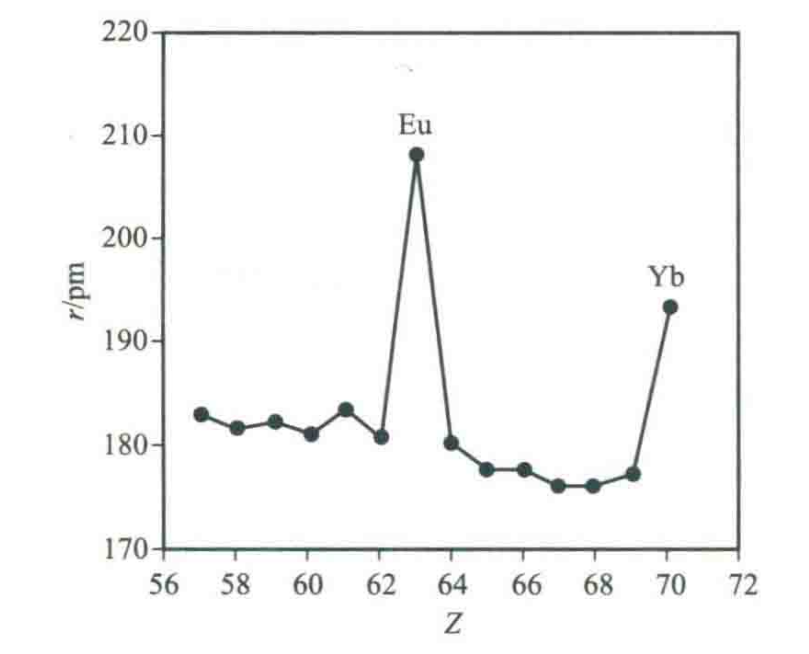
\includegraphics[width=0.5\textwidth]{figure//双峰效应1.png}
	\caption{原子半径的骤升}
	\label{fig:}
\end{figure}

\begin{figure}[htpb]
	\centering
	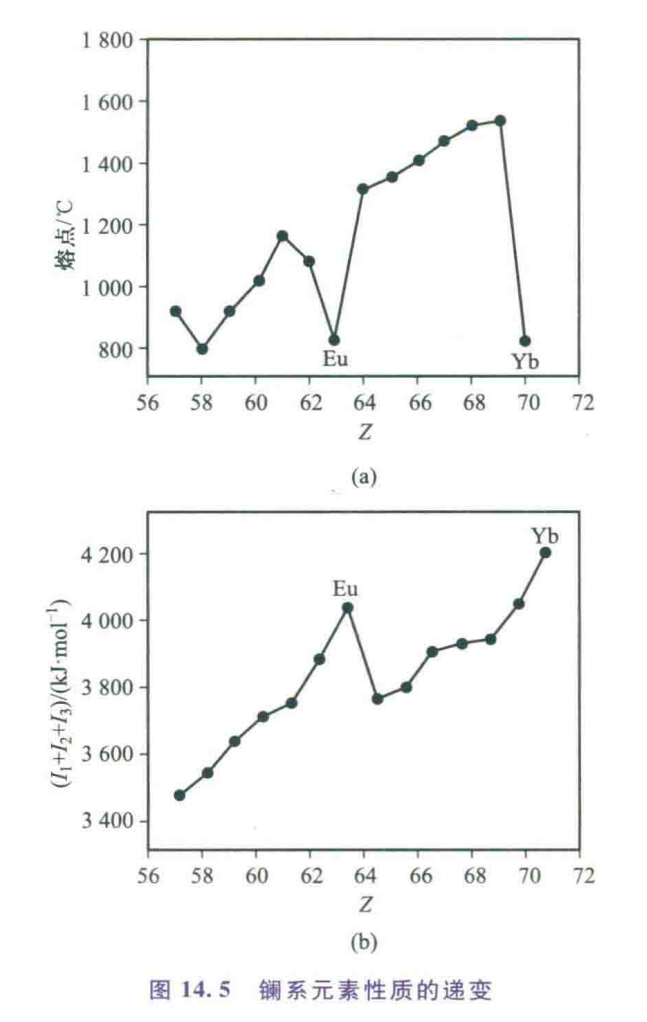
\includegraphics[width=0.5\textwidth]{figure//双峰效应2.png}
	\caption{熔点和一二三电离能总和的“双峰”}
	\label{fig:}
\end{figure}

2.离子半径

与原子半径变化不同,\ce{Ln^3+}的离子半径变化十分有规律,这也导致它们性质极为相似,造成分离上的困难。\\

钇组元素:由于镧系收缩,\ce{Eu}以后的元素性质接近\ce{Y},它们在自然界中共生。\\

\subsubsection{金属活泼性}

镧系元素单质都十分活泼,活泼性与镁相近,且活泼性随着原子序数的增大稍有下降。

与空气反应:金属在空气中被缓慢氧化,加热则容易燃烧,生成\ce{Ln2O3},\ce{Ce}则生成\ce{CeO2}。

与水反应:镧系金属均可与水反应,尤其是热水,反应放出氢气。

与非金属反应:镧系金属可以与大部分非金属反应,反应一般不很剧烈。与卤素加热燃烧生成\ce{LnX3},与氢气加热生成\ce{LnH2}或\ce{LnH3},它们一般属于金属型氢化物。

锕系元素很活泼,它们与沸水作用同时生成氧化物和氢氧化物。它们均可被氢氟酸侵蚀,但大多数仅缓慢与硝酸反应,不与碱发生反应。

\subsubsection{离子的颜色}

按照晶体场理论,f轨道也会发生分裂,当其处于部分填充时,也会发生f-f跃迁,\ce{Ln^3+}的颜色主要由f-f跃迁引起,所以,离子的颜色主要与未成对的f电子数有关。

\subsubsection{离子的磁性}

仅有\ce{La^3+}和\ce{Lu^3+}的未成对电子数为0反磁性,其余均为顺磁性。

\subsection{镧系元素的重要化合物}

\subsubsection{Ln(III)的化合物}

镧系元素化合物体积大,且4f电子被遮蔽,大部分镧系化合物是离子型的。

1.氧化物和氢氧化物

可形成\ce{Ln2O3},颜色与对应离子颜色一致,离子型化合物,熔点很高,均具有碱性,难溶于水,易溶于酸,能形成碱式碳酸盐。

2.盐类

镧系卤化物中仅有\ce{LnF3}不溶于水。

若要制得无水\ce{LnCl3}则需在\ce{HCl}气流中或者过量\ce{NH4Cl}存在下加热。

3.配合物

除了水合离子之外,\ce{Ln^3+}形成配合物的能力不是很强,因为4f被5s,5p轨道屏蔽,离子形成稀有气体结构。又由于半径大,所以配位数一般在6或6以上。

\ce{Ln^3+}与冠醚形成稳定配合物。

\subsection{稀土元素}

稀土元素化学性质活泼,可以溶于碱金属氯化物,与水作用放出氢气。

\subsubsection{稀土元素的应用}

1.冶金工业上,可用于脱氧脱硫,克服氢脆,增加强度,总之牛逼就完事了。

2.汽车和石油化工上,用作废气催化剂或裂化催化剂。

3.做特种玻璃。

4.荧光体和激光材料。

5.制陶业,增强性能,牛逼。

6.电子工业上,用作永磁体。

7.农业上用作化肥,金坷垃牛逼炸了。

\end{document}
